\documentclass[english, a4paper]{article}

\usepackage[T1]{fontenc}    % Riktig fontencoding
\usepackage[utf8]{inputenc} % Riktig tegnsett
\usepackage{babel}          % Ordelingsregler, osv
\usepackage{graphicx}       % Inkludere bilder
\usepackage{booktabs}       % Ordentlige tabeller
\usepackage{url}            % Skrive url-er
\usepackage{textcomp}       % Den greske bokstaven micro i text-mode
\usepackage{units}          % Skrive enheter riktig
\usepackage{float}          % Figurer dukker opp der du ber om
\usepackage{lipsum}         % Blindtekst
\usepackage{subcaption} 
\usepackage{color}
\usepackage{amsmath}  
\usepackage{amssymb}
\usepackage{hyperref}
\usepackage{pagecolor}
%\usepackage{minted}
\usepackage{braket} 
\usepackage{multicol}
\usepackage{listings}    %Add source code
\usepackage{amsfonts}
\usepackage{setspace}
\usepackage[cm]{fullpage}		% Smalere marger.
\usepackage{verbatim} % kommentarfelt.
\usepackage{tabularx}
\usepackage{booktabs}
\usepackage{tikz}				

\usetikzlibrary{shapes,arrows}	
\usetikzlibrary{arrows,decorations.markings}

\definecolor{decisionColor}{HTML}{DEE1B2}
\definecolor{nodeColor}{HTML}{B2DFE2}

\tikzstyle{roundrect}=[rectangle, rounded corners, minimum width=3cm, minimum height=1cm, text centered, draw=black, fill=nodeColor, text width=3.5cm] 
\tikzstyle{decision} = [diamond, minimum width=3.7cm, minimum height=3.2cm, text centered, draw=black, fill=decisionColor, scale=1, text width=2.05cm]
\tikzstyle{arrow} = [decoration={markings,mark=at position 1 with
	{\arrow[scale=1.5,>=stealth]{>}}},postaction={decorate}]

\setlength{\columnseprule}{1pt}	%(width of separationline)
\setlength{\columnsep}{1.0cm}	%(space from separation line)
\newcommand\lr[1]{\left(#1\right)} 
\newcommand\bk[1]{\langle#1\rangle} 
\newcommand\uu[1]{\underline{\underline{#1}}} % Understreker dobbelt.
\newcolumntype{Y}{>{\centering\arraybackslash}X}
\definecolor{qc}{rgb}{0,0.4,0}
\definecolor{LightBlue}{rgb}{0.8, 0.8, 0.9}
\hypersetup{
	colorlinks,
	linkcolor={red!30!black},
	citecolor={blue!50!black},
	urlcolor={blue!80!black}
}
% JF i margen
\makeatletter
\renewcommand{\subsubsection}{\@startsection{subsubsection}{3}{0pt}%
	{-\baselineskip}{0.5\baselineskip}{\bf\large}}
\makeatother
\newcommand{\jf}[1]{\subsubsection*{JF #1}\vspace*{-2\baselineskip}}

\newcommand{\bm}[1]{\mathbf{#1}}

% Skru av seksjonsnummerering (-1)
\setcounter{secnumdepth}{3}

\begin{document}
	%\pagecolor{black!50!}
	\renewcommand{\figurename}{Figure}
	% Forside
	\begin{titlepage}
		\begin{center}
			
			\textsc{\Large FYS4411 - Computational quantum mechanics }\\[0.5cm]
			\textsc{\Large Spring 2016}\\[1.5cm]
			\rule{\linewidth}{0.5mm} \\[0.4cm]
			{ \huge \bfseries  Project 2;\\ Variational Monte Carlo studies of electronic systems}\\[0.10cm]
			\rule{\linewidth}{0.5mm} \\[1.5cm]
			
			{\Large Github repository:} \\*[0.4cm]
			\url{https://github.com/filiphl/FYS4411.git}
			
			\vspace{13.5cm}
			
			% Av hvem?
			
			\begin{minipage}{\textwidth}
				\begin{minipage}{0.333\textwidth}
					\begin{center} \large
						Sean Bruce Sangolt Miller\\
						{\footnotesize s.b.s.miller@fys.uio.no}
					\end{center}
				\end{minipage}
				\quad
				\begin{minipage}{0.333\textwidth}
					\begin{center} \large
						Filip Henrik Larsen\\
						{\footnotesize filiphenriklarsen@gmail.com}
					\end{center}
				\end{minipage}
				\quad
				\begin{minipage}{0.333\textwidth}
					\begin{center} \large
						Roar Emaus\\
						{\footnotesize 
						roarem@fys.uio.no}
					\end{center}
				\end{minipage}
			\end{minipage}
		
			\vfill
			
			% Dato nederst
			\large{Date: \today}
			
		\end{center}
	\end{titlepage}
	%%%%%%%%%%%%%%%%%%%%%%%%%%%%%%%%%%%
	
	\begin{abstract}
		
	\end{abstract}
	
	
	%%%%%%%%%%%%%%%%%%%%%%%%%%%%%%%%%%%
	\pagenumbering{gobble}% Remove page numbers (and reset to 1)
	\tableofcontents
	\newpage
	\pagenumbering{arabic}% Arabic page numbers (and reset to 1)
	%\begin{multicols*}{2}
	
	
	\section{Introduction}
	Quantum dots are, possibly large, atomic systems packed so closely together that the Pauli principle forces the electrons to be in different states. These systems can be made approximately 2-dimensional\footnote{I.e. all electron movement is confined to a plane. This does not mean the space is considered two-dimensional, so the 3-dimensional Coulomb potential will still be used.} by strings of quantum dots. Quantum dots are much larger than atoms while possessing many of their characteristics, which means they are both easy and interesting to measure. Measurements provide means with which to test quantum theory and models.\\
	Up to 20 electrons, it is reasonable to approximate the system Hamiltonian by placing all electrons in a harmonic oscillators and having coulomb interactions. If only closed-shell quantum dots are considered, a model that splits the wavefunction can be used, which greatly reduces the number of calculations. The purpose of this project is see if this simple model can reproduce known results. This will be done through variational Monte-Carlo (VMC) by using a Slater determinant with a Pade-Jastrow factor\\
	First, a detailed calculation of the two-body quantum dot will be performed, followed by deduction of algorithms for a general many-body numerical approach to a system of $N=\{2,\:6,\:12,\:20\}$ electrons. Then, an explanation of the optimization of the variational parameters will given, followed by a small talk on the "blocking" method. Since the program script will be large, a few benchmarks will be mentioned. Lastly, results will be presented followed by some comments.
	
	\section{Theory and Methods}
	\subsection{Preliminary derivations}
	While performing VMC it is of course favourable to use analytical expressions, should they not demand an unacceptable increase in CPU time. We will therefore need to calculate the local energy $E_L = \frac{1}{\Psi_T}H\Psi_T$ and the quantum force $F = \frac{2}{\Psi_T}\nabla\Psi_T$. The Hamiltonian $H$ used will be:
	
	\begin{equation}
	H = H_0 + H_I = \sum_{i=1}^{N}\left(-\frac{1}{2}\nabla_i^2 + \frac{1}{2}\omega^2r_i^2\right) + \sum_{i<j}\frac{1}{r_{ij}}
	\end{equation}
	
	I.e. a harmonic oscillator potential with Coulomb interactions. The Laplacian will be the most demanding quantity to calculate.
	
	\subsection{Singlet electron state}
	For an electron in a harmonic oscillator potential, the energy is given by $\epsilon_n = \omega(n + 1)$, where we have used natural units and $n = n_x + n_y + \ldots$. For two non-interacting electrons, the energy is $\epsilon_{n_1,n_2} = \omega(n_{x,1} + n_{y,1} + \ldots + n_{x,2} + n_{y,2} + \ldots + 2)$. Obviously the energy is lowest for $n_1 = n_2 = 0$, giving $\epsilon_{0,0} = 2\omega$.\\
	Since $n_1=n_2 = 0$ means the two electron are in the same spatial wavefunction, they must have different spins. 
	Since electrons are spin-$\frac{1}{2}$ particles, they combine to give total spin zero, i.e. they form the singlet state.\\
	
	For the singlet electron state we will use the trial wavefunction:
	
	\begin{equation}
	\Psi_T(\bm{r}_1,\bm{r}_2) = Ce^{-\frac{\alpha\omega}{2}(r_1^2+r_2^2)}e^{\frac{ar_{12}}{1+\beta r_{12}}}\quad,\quad a=1 \label{TwoBodyTrailWavefunction}
	\end{equation}
	
	The Laplacian of which (for particle $i$) is:
	
	\begin{equation}
	\nabla_i^2 \Psi_T = \nabla_i(\nabla_i\Psi_T)
	\end{equation}
	
	We will use the following change of coordinates when it simplifies calculations:
	
	\begin{align}
	\begin{split}
	\frac{\partial}{\partial r_{i,j}} &= \frac{\partial r_{12}}{\partial r_{i,j}}\frac{\partial}{\partial r_{12}}\\
	\rightarrow \nabla_i &= \frac{(-1)^i}{r_{12}}(x_1-x_2, y_1-y_2)\frac{\partial}{\partial r_{12}}\\
	&= \frac{(-1)^i}{r_{12}}\bm{r}_{12}\frac{\partial}{\partial r_{12}}
	\end{split}
	\label{eq:coord_change_nabla}
	\end{align}
	
	where $r_{i,j}$ is element $j$ of $\bm{r}_i$.
	The gradient, which is needed for the quantum force as well, is then
	
	\begin{align}
	\begin{split}
	\nabla_i\Psi_T &= -\alpha\omega\bm{r}_i\Psi_T + \frac{(-1)^i}{r_{12}}\bm{r}_{12}\left[\frac{\partial}{\partial r_{12}}\left(\frac{ar_{12}}{1+\beta r_{12}}\right)\right]\Psi_T\\
	&= \left[-\alpha\omega\bm{r}_i + \frac{(-1)^i}{r_{12}}\bm{r}_{12}\frac{a}{(1+\beta r_{12})^2}\right]\Psi_T
	\end{split}
	\label{eq:grad_singlet}
	\end{align} 
	
	which means the Laplacian is
	
	\begin{equation}
	\begin{split}
	\nabla_i^2\Psi_T &= \left[\nabla_i[\ldots]\right]\Psi_T + [\ldots]\nabla_i\Psi_T\\
	&= \left[\nabla_i[\ldots]\right]\Psi_T + [\ldots]^2\Psi_T
	\end{split}
	\end{equation}
	
	where $[\ldots]$ is the last parenthesis in equation \ref{eq:grad_singlet}. The parenthesis in the first term above is
	
	\begin{align}
	\begin{split}
	\nabla_i\left[-\alpha\omega\bm{r}_i + \frac{(-1)^i}{r_{12}}\bm{r}_{12}\frac{a}{(1+\beta r_{12})^2}\right] &= -2\alpha\omega + \frac{(-1)^i}{r_{12}}\left( \frac{(-1)^i2ar_{12}}{(1+\beta r_{12})^2} - \frac{(-1)^i2a\beta r_{12}}{(1+\beta r_{12})^3} - \frac{(-1)^ia}{r_{12}(1+\beta r_{12})^2}\right)\\
	&= -2\alpha\omega - \frac{a}{(1+\beta r_{12})^2}\left( \frac{1}{r_{12}} - \frac{2}{r_{12}} + \frac{2\beta}{1+\beta r_{12}}\right)\\
	&= -2\alpha\omega + \frac{a}{r_{12}(1+\beta r_{12})^2}- \frac{2a\beta}{(1+\beta r_{12})^3}
	\end{split}
	\end{align}
	
	which gives
	
	\begin{equation}
	\nabla_i^2\Psi_T = \left[-2\alpha\omega + \frac{a}{r_{12}(1+\beta r_{12})^2} - \frac{2a\beta}{(1+\beta r_{12})^3} + \alpha^2\omega^2r_i^2 + \frac{a^2}{(1+\beta r_{12})^4} - \frac{2\alpha\omega a(-1)^i}{r_{12}(1+\beta r_{12})^2}\bm{r}_i\cdot\bm{r}_{12}\right] \Psi_T
	\end{equation}
	
	We therefore have:
	
	\begin{equation}
	\sum_{i=1}^2\frac{1}{\Psi_T}\nabla_i^2\Psi_T = -4\alpha\omega + \frac{2a}{r_{12}(1+\beta r_{12})^2} - \frac{4a\beta}{(1+\beta r_{12})^3} + \alpha^2\omega^2(r_1^2 + r_2^2) + \frac{2a^2}{(1+\beta r_{12})^4} - \frac{2\alpha\omega a}{(1+\beta r_{12})^2}r_{12}
	\end{equation}
	
	\subsection{Closed, 2-dimensional shell states}
	If we again consider the non-interacting, harmonic oscillator confined electron system, we can increase the number of electrons beyond 2. If, in some wondrous universe, we had fermions with three different spins states (like a spin-1 boson), then for three electrons we could again set $n_1=n_2=n_3 = 0$ and have an anti-symmetric spin state. However, in our world, we must go up in energy for more than two electrons.\\
	The $n=0$ state was the ground state. The next state has degeneracy 2; $(n_1,n_2) = (1,0), (0,1)$. After that we have degeneracy 3;$(n_1,n_2) = (2,0), (1,1), (0,2)$. Each of these states are doubly degenerate due to spin.\\
	
	The reason in explaining this is because, assuming we have a so-called "closed shell" problem\footnote{For every new tier in energy, we fill it up with electrons. So all considered tiers, or "shells", are full (or "closed")}, we can do some manipulations that greatly reduce the number of calculations necessary to perform VMC. Firstly, we need to rewrite the trial wavefunction.\\
	As is already known, the true wavefunction is approximated by an analytical solution to some simpler problem, and a Jastrow factor. The analytical part can be written as a Slater determinant:
	
	\begin{equation}
	\Psi_{D} = \frac{1}{\sqrt{N}}
	\begin{vmatrix}
	\phi_1(\bm{r}_1) & \phi_2(\bm{r}_1) & \ldots & \phi_{N-1}(\bm{r}_1) & \phi_N(\bm{r}_1)\\
	\phi_1(\bm{r}_2) & \phi_2(\bm{r}_2) & \ldots & \phi_{N-1}(\bm{r}_2) & \phi_N(\bm{r}_2)\\
	& & \vdots & &\\
	\phi_1(\bm{r}_N) & \phi_2(\bm{r}_N) & \ldots & \phi_{N-1}(\bm{r}_N) & \phi_N(\bm{r}_N)\\
	\end{vmatrix}
	\end{equation}
	
	and therefore our trial wavefunction will be:
	
	\begin{equation}
	\Psi_T = \Psi_{D}\Psi_{C} \:\:,\:\: \Psi_{C} = \prod_{i<j}^N e^{f_{ij}}\quad,\quad f_{ij} \equiv\frac{a_{ij}r_{ij}}{1+\beta r_{ij}} \label{ManyBodyWavefunction}
	\end{equation}
	
	where $\alpha$, $\beta$ are the variational parameters, $a_{ij}$ is connected to particle spins, and $N$ is the total number of particles. The single particle functions are solutions to the two dimensional, harmonic oscillator Scr\"odinger equation:
	
	\begin{equation}
	\phi_i(\bm{r_i}) = C H_{n_{x,i}}(\sqrt{\omega \alpha}x_i)H_{n_{y,i}}(\sqrt{\omega \alpha}y_i)e^{\frac{\omega\alpha}{2}r_i^2}
	\end{equation}
	
	Obviously, $\Psi_{D}$ is a time consuming object to calculate at every Metropolis step. We will therefore do some neat tricks that reduce the number of calculations.\\
	The first is to rewrite $\Psi_D$ by using that the Hamiltonian is spin-independent. If we now let $\phi_n$ be the spatial-component of the wavefunction, then it causes no effect on the energy if we write:
	
	\begin{equation}
		\Psi_T = \Psi_{D+}\Psi_{D-}\Psi_C
	\end{equation}
	
	where $\Psi_{D+} \equiv |D_+|$ and $\Psi_{D-} \equiv |D_-|$ are Slater determinants consisting only of spin-up and spin-down particles, respectively. This means $|D_+|$ and $|D_-|$ are $\frac{N}{2}$-dimensional, and we see this method only works for closed shell systems. We will let the first $\frac{N}{2}$ particles be spin-up and the rest spin-down. That is, $\bm{r_1}-\bm{r}_{N/2}$ are the positions of the spin-up particles, while the rest are positions for spin-down particles. Obviously this is wrong, since we can't separate which particles are spin-up and which are spin-down in reality, due to the properties of identical particles. However, as stated, due to the spin-independent Hamiltonian, this causes no effect on the energy, which is all we're after.
	
	\subsection{The Metropolis ratio test}
	The basic principle behind the Metropolis algorithm is to make an assumption on the transition probability for a system to move from setting to another, as
	an exact, or even approximate, expression is lacking.
	
	If the probability distribution for a state $i$ is given by $w_i$, then from Markov chain theory the time derivative is:
	
	\begin{align}
		\frac{\partial w_i(t)}{\partial t} = \sum_j W(j\rightarrow i)w_j(t) - W(i\rightarrow j)w_i(t)
	\end{align}
	
	where $W_{i\rightarrow j}$ is the probability of moving from a state $i$ to another state $j$, i.e the rate of change in $w_i$ is given by the probability for a state $j$ to go to $i$ minus the
	probability of state $i$ going to $j$, summed over all $j$.
	The most likely state will fulfil $\frac{\partial w_i(t)}{\partial t} = 0$, giving:
	
	\begin{align}
		\begin{split}
			W(j\rightarrow i)w_j(t) &=  W(i\rightarrow j)w_i(t)\\
			\Rightarrow\:\:\:\frac{  W(j\rightarrow i)}{  W(i\rightarrow j)} &= \frac{w_i}{w_j}
		\end{split}
	\end{align}
	
	Since the transition probability $W$ is unknown, we approximate it by guessing its form:
	
	\begin{align}
		W(j\rightarrow i) &= T(j\rightarrow i) A(j\rightarrow i)
	\end{align}
	
	where $T$ is the transition moving probability, while $A$ is the probability of accepting such a move. Furthermore, in brute force Metropolis, one guesses $T_{i\rightarrow j} = T_{j\rightarrow i}$.
	Therefore:
	
	\begin{equation}
		\frac{A_{j\rightarrow i}}{A_{i\rightarrow j}} = \frac{w_i}{w_j}
	\end{equation}
	
	Since the probability densities are known, it is known whether or not this ratio is larger than one. If it's larger than one, then the acceptance probability from $j$ to $i$ is the biggest, i.e we are more likely to accept the move than not.
	Therefore, we simply say the move is accepted. However, if the probability ratio is smaller than one, then we are more likely to move from the new state to the one the system is currently in.
	To check whether or not we should accept the move, we may compare it to, say, a ``coin toss''; if it's bigger, the move is accepted.\\
	
	So, at each Metropolis step, we need the ratio of probabilities. We first define $R\equiv\frac{\Psi_T^n}{\Psi_T^o}$, where "$n$" means the new wavefunction and "$o$" means the old (or the current, but "c" could be confused with "correlation"). Written out, this is:
	
	\begin{equation}
	R = \frac{|D_+^n|}{|D_+^o|}\frac{|D_-^n|}{|D_-^o|}\frac{\Psi_C^n}{\Psi_C^o}
	\end{equation}
	
	If we only move one position at a time, then only one row in either $D_+$ or $D_-$ will change. This means if we move a spin-up position, then $|D_-^n| = |D_-^o|$, so we need only consider one of the determinant fractions for each $R$.\\
	Through some simple steps, one can show the determinant fraction ($R_{D}$) reduces to:
	
	\begin{equation}
	R_D = \sum_{j=1}^{N/2} D_{ij}(\bm{r}^n)D_{ji}^{-1}(\bm{r}^o)
	\end{equation}
	
	where $D_{ij}^{-1}$ is element\footnote{Where $i$ is the row and $j$ is the column.} $ij$ of the inverse of $D$, $D$ is either the spin-up or spin-down determinant, and $\bm{r}_i$ is the moved position. Since $D_{ij}(\bm{r}) = \phi_j(\bm{r}_i)$, the only difficulty remaining is to find the elements of the inverse matrix.\\
	
	The elements of an inverse matrix are given by the Sherman-Morrison formula, which, when applied to the current case, gives:
	
	\begin{equation}
	D_{kj}^{-1}(\bm{r}^n) =
	\begin{cases}
	D_{kj}^{-1}(\bm{r}^o) - \frac{D_{ki}^{-1}(\bm{r^o})}{R_D}\sum_{l=1}^{N/2}D_{il}(\bm{r}^n)D_{lj}^{-1}(\bm{r}^o) \:&\text{if}\: j\neq i\\ \vspace{1pt}\\
	\frac{D_{ki}^{-1}(\bm{r^o})}{R_D} \:&\text{if}\: j = i \\
	\end{cases}
	\label{eq:update_inverse_SD}
	\end{equation}
	
	The ratio for the correlation function has a rather nice expression:
	
	\begin{align}
	\begin{split}
	\frac{\Psi_C^n}{\Psi_C^o} &= \prod_{i<j}^{N/2} e^{(f_{ij}^n-f_{ij}^o)}\\
	&= \exp\left( \sum_{i<j}^{N/2} f_{ij}^n - f_{ij}^o \right)\\
	&= \exp\left(\sum_{i=0}^{k-1}(f_{ik}^n - f_{ik}^o) + \sum_{j=k+1}^{N/2}(f_{kj}^n - f_{kj}^o)\right)
	\end{split}
	\end{align}
	
	were we used $f_{ij}^n-f_{ij}^o=0\:\forall\:i,j\neq k$, and $k$ is the moved position. The first sum is then for $j=k$ and the second sum is for $i=k$, with the restriction $i<j$.\\
	The only step that remains is to square and multiply the two ratios\footnote{Or multiply and then square. Really, it's up to you.}.
	
	\subsection{Importance sampling}
	In importance sampling, each suggested move requires the calculation of the quantum force:
	
	\begin{equation}
	x_{new} = x_{old} + DF(x_{old})\Delta t + \xi\sqrt{\Delta t}
	\end{equation}
	
	Solutions to the Fokker-Planck equation gives the transition probability, which must be multiplied with the probability density. The transition probability is therefore given by:
	
	\begin{equation}
	G(y,x,\Delta t) = \frac{1}{(4\pi D\Delta t)^{3N/2}}\exp\left\{ -\frac{(y-x-D\Delta tF(x))^2}{4D\Delta t} \right\}
	\end{equation}
	
	where $y$ is the new position and $x$ the old, and the acceptance test becomes:
	
	\begin{equation}
	q(y,x) = \frac{G(x,y,\Delta t)|\Psi_T(y)|^2}{G(y,x,\Delta t)|\Psi_T(x)|^2}
	\end{equation}
	
	The quantum force, given by $F = 2\frac{\nabla \Psi_T}{\Psi_T}$, requires the gradient of $\Psi_T$. Obviously, the quantum force can be written\footnote{The superscript "o" has been dropped since there will be no "mix" of new and old coordinates for the rest of this subsection.}:
	
	\begin{equation}
	F = 2\left(\frac{\nabla |D_+|}{|D_+|} + \frac{\nabla |D_-|}{|D_-|} + \frac{\nabla \Psi_C}{\Psi_C}\right)
	\end{equation}
	
	Of course, when only position $k$ is altered, only the $k$'th gradient in $\nabla$ changes (recall the definition $\nabla \equiv (\nabla_1, \nabla_2, \ldots, \nabla_N$), and needs to be re-evaluated. We know the determinant can written:
	
	\begin{equation}
	|D| = \sum_{j=1}^{N/2}D_{kj}C_{jk}
	\end{equation}
	
	where $C_{jk}$ are the cofactors of $D$, and is independent of the $i$'th row in $D$, i.e. changing $k$ does not change $C_{jk}$. It is therefore independent of the position change. Changing row $i$ means all the other gradients in $\nabla|D|$ are the same as before, and we only need to re-evaluate $\nabla_k|D|$. This means:
	
	\begin{align}
	\begin{split}
	\frac{\nabla_k|D|}{|D|} &= \frac{\nabla_k\sum_{j=1}^{N/2}D_{kj}C_{jk}}{|D|}\\
	&= \sum_{j=1}^{N/2}\frac{(\nabla_kD_{kj})C_{jk}}{|D|}\\
	&= \sum_{j=1}^{N/2}(\nabla_kD_{kj})D_{jk}^{-1}
	\end{split}
	\end{align}
	
	which, from equation \ref{eq:update_inverse_SD}, means:
	
	\begin{equation}
	\frac{\nabla_k|D^n}{|D^n|} = \frac{1}{R_D}\sum_{j=1}^{N/2}(\nabla_kD_{kj}^n)(D_{jk}^o)^{-1}
	\end{equation}
	
	where the factor $\nabla_kD_{kj} = \nabla_k \phi_j(\bm{r}_k)$ is:
	
	\begin{align}
		\begin{split}
		\nabla_kD_{kj} = A\Big(&H_{n_{j,x}}'(\sqrt{\omega\alpha}x_k)H_{n_{j,y}}(\sqrt{\omega\alpha}y_k) - \alpha\omega x_kH_{n_{j,x}}(\sqrt{\omega\alpha}x_k)H_{n_{j,y}}(\sqrt{\omega\alpha}y_k)\\
		,&H_{n_{j,y}}'(\sqrt{\omega\alpha}y_k)H_{n_{j,x}}(\sqrt{\omega\alpha}x_k) - \alpha\omega y_kH_{n_{j,x}}(\sqrt{\omega\alpha}x_k)H_{n_{j,y}}(\sqrt{\omega\alpha}y_k)\Big)e^{-\frac{\alpha\omega}{2}r_k^2}
		\end{split}
	\end{align}

	The correlation function gradient can be expressed:
	
	\begin{align}
	\begin{split}
	\frac{\nabla_k \Psi_C}{\Psi_C} &= \frac{1}{\Psi_C}\nabla_k e^{\sum_{i<j}^Nf_{ij}}\\
	&= \sum_{i=1}^{k-1}\nabla_kf_{ik} + \sum_{j=k+1}^{N}\nabla_kf_{kj}
	\end{split}
	\end{align}
	
	but since $f_{ij}$ only depends on $r_{ij}$, it would preferable to express $\nabla_k$ in terms of $r_{ij}$. In equation \ref{eq:coord_change_nabla}, we showed this change for a simpler system. Applied to this problem, we can derive:
	
	\begin{align}
	\begin{split}
	\nabla_k &=  \frac{1}{r_{ik}}\bm{r}_{ik}\frac{\partial}{\partial r_{ik}}\\
	&\text{or}\\
	\nabla_k &=  -\frac{1}{r_{jk}}\bm{r}_{jk}\frac{\partial}{\partial r_{jk}}
	\end{split}
	\end{align}
	
	which gives:
	
	\begin{equation}
	\frac{\nabla_k \Psi_C}{\Psi_C} = \sum_{i=1}^{k-1}\frac{\bm{r}_{ik}}{r_{ik}}\frac{\partial f_{ik}}{\partial r_{ik}} - \sum_{j=k+1}^{N}\frac{\bm{r}_{kj}}{r_{kj}}\frac{\partial f_{kj}}{\partial r_{kj}}
	\end{equation}
	
	We now have all the necessary tools to perform importance sampling.
	
	\subsection{Local energy}
	Lastly, the local energy needs to be calculated. As usual, the Laplacian fraction $\frac{\nabla^2\Psi_T}{\Psi_T}$ is the most demanding object to calculate. the starting point is:
	
	\begin{equation}
	\frac{\nabla^2\Psi_T}{\Psi_T} = \frac{\nabla^2 |D_+|}{|D_+|} + \frac{\nabla^2 |D_-|}{|D_-|} + \frac{\nabla^2 \Psi_C}{\Psi_C} + 2\left( \frac{\nabla |D_+|}{|D_+|} + \frac{\nabla |D_-|}{|D_-|} \right)\cdot\frac{\nabla \Psi_C}{\Psi_C}
	\end{equation}
	
	which looks easy enough. The last term contain vectors already known, while the first two are derived in the exact same manner as for the gradients, i.e.
	
	\begin{equation}
	\frac{\nabla_k^2|D|}{|D|} = \sum_{j=1}^{N/2}(\nabla_k^2D_{kj})D_{jk}^{-1}
	\end{equation}
	
	where (here we abbreviate $H_{n_{j,z}}(\sqrt{\omega\alpha}z_k)$ by $H_{n_j}(z)$ for compactness)
	
	\begin{align}
		\begin{split}
		\nabla_k^2D_{kj} = A\Big[&H_{n_j}''(x)H_{n_j}(y) + H_{n_j}''(y)H_{n_j}(x)\\
		&- 2\alpha\omega\left(xH_{n_j}'(x)H_{n_j}(y) + yH_{n_j}'(y)H_{n_j}(x)\right)\\
		&- \alpha\omega H_{n_j}(x)H_{n_j}(y)\left(d - \alpha\omega r_k^2\right)\Big]e^{-\frac{\alpha\omega}{2}r_k^2}
		\end{split}
	\end{align}
	
	Unfortunately, the middle term is not so nice to find. The steps needed are many and tedious, but not difficult. They are therefore omitted and we show only the final result:
	
	\begin{equation}
	\frac{\nabla_k^2 \Psi_C}{\Psi_C} = \left(\frac{\nabla_k\Psi_C}{\Psi_C}\right)^2 + \sum_{i=1}^{k-1}\left[\frac{d-1}{r_{ik}}\frac{\partial f_{ik}}{\partial r_{ik}} + \frac{\partial^2 f_{ik}}{\partial r_{ik}^2}\right] + \sum_{j=k+1}^{N}\left[\frac{d-1}{r_{kj}}\frac{\partial f_{kj}}{\partial r_{kj}} + \frac{\partial^2 f_{kj}}{\partial r_{kj}^2}\right]
	\end{equation}
	
	where $d$ is the dimension we consider and:
	
	\begin{align}
	\frac{\partial f_{ij}}{\partial r_{ij}} &= \frac{a_{ij}}{(1+\beta r_{ij})^2}\\
	\frac{\partial^2 f_{ij}}{\partial r_{ij}^2} &= -\frac{2a_{ij}\beta}{(1+\beta r_{ij})^3}
	\end{align}
	
	where $a_{ij}$ equals $1$ for anti-parallel spins and $\frac{1}{3}$ for parallel.
	
	
	\subsection{Flowchart of metropolis algorithm}
	\begin{figure}[H]
		\begin{center}
			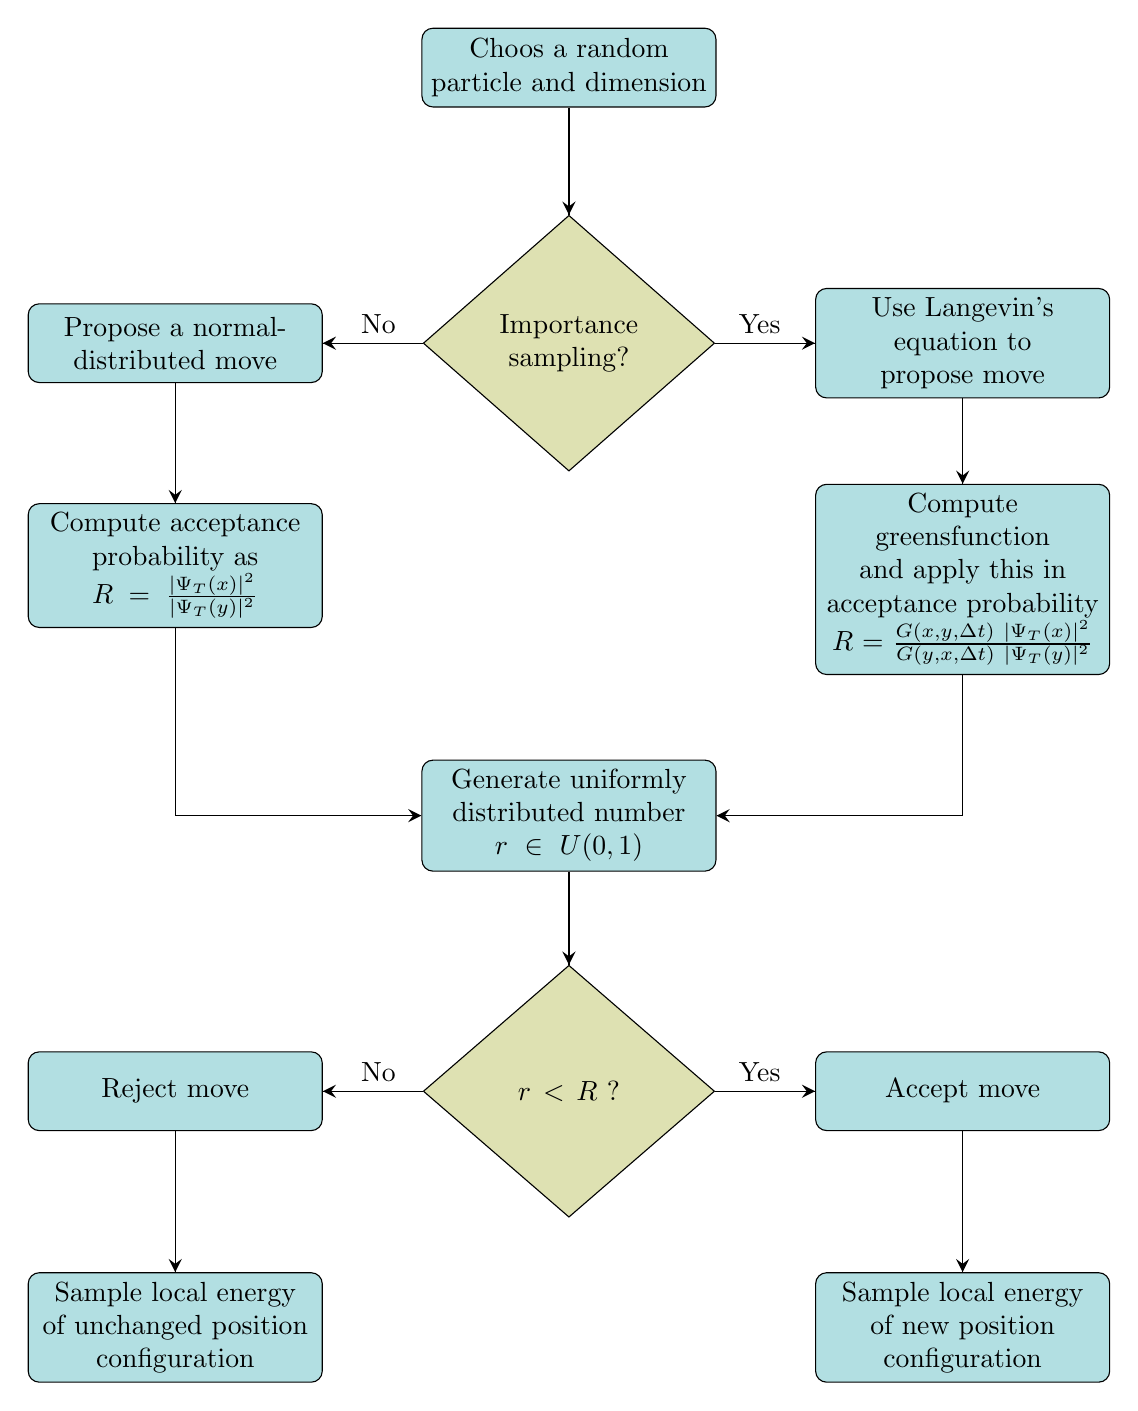
\begin{tikzpicture} [node distance=3cm]
			\node (particleAndDimension) [roundrect] {Choos a random particle and dimension};% of one particle in one dimension};
			
			\node (importance test)[decision, below of=particleAndDimension, yshift=-0.5cm]{Importance sampling?};
			
			\node (Langevin) [roundrect,right of=importance test, xshift=2cm] {Use Langevin's equation to propose move};
			\node (importance ratio) [roundrect,below of=Langevin] {
				Compute greensfunction and apply this in acceptance probability\\
				$R = \frac{G(x,y,\Delta t)~|\Psi_T(x)|^2}{G(y,x,\Delta t)~|\Psi_T(y)|^2}$};
			
			\node (unimportant move) [roundrect,left of=importance test, xshift=-2cm] {
				Propose a normal-distributed move};
			\node (standard ratio) [roundrect,below of=unimportant move, yshift=0.5em] {
				Compute acceptance probability as
				$R = \frac{|\Psi_T(x)|^2}{|\Psi_T(y)|^2}$};
			
			\node (random number)[roundrect, below of=importance test, yshift=-3.0cm]{
				Generate uniformly distributed number\\
				$r\in U(0,1)$	
			};
			\node (Accept)[decision, below of=random number, yshift=-0.5cm]{
				$r<R$~?
			};
			
			\node (Accepted) [roundrect,right of=Accept, xshift=2cm] {Accept move};
			\node (New sample)[roundrect,below of=Accepted]{Sample local energy of new position configuration};
			
			
			\node (Rejected) [roundrect,left of=Accept, xshift=-2cm] {Reject move};
			\node (Old sample)[roundrect,below of=Rejected]{Sample local energy of unchanged position configuration};
			
			
			
			\draw [arrow] (particleAndDimension) -- (importance test);
			\draw [arrow] (importance test) -- node [anchor=south, xshift=-0.2em]{Yes} (Langevin);
			\draw [arrow] (Langevin) --(importance ratio);
			\draw [arrow] (importance ratio) |- (random number) ;
			\draw [arrow] (importance test) -- node [anchor=south, xshift=0.2em]{No} (unimportant move);
			\draw [arrow] (unimportant move) -- (standard ratio);
			\draw [arrow] (standard ratio) |- (random number);
			\draw [arrow] (random number) -- (Accept);
			\draw [arrow] (Accept) -- node [anchor=south, xshift=-0.2em]{Yes} (Accepted);
			\draw [arrow] (Accept) -- node [anchor=south, xshift=0.2em]{No} (Rejected);
			\draw [arrow] (Accepted) -- (New sample);
			\draw [arrow] (Rejected) -- (Old sample);
			
			\end{tikzpicture}
		\end{center}
	\end{figure}
	
	
	
	\subsection{Optimizing parameters}
	Our trial wavefunctions, both for the two-body system and many-body system (equations \ref{TwoBodyTrailWavefunction} and \ref{ManyBodyWavefunction}), contain two variational parameters, $\alpha$ and $\beta$.
	In the VMC approach, the minimal energy is sought. Therefore, the goal is to minimize $\langle E_L\rangle$ with respect to these variational parameters.
	There are several ways to minimize a value with respect to some parameters, and here we will use the method of steepest descent (SD). The SD method, in algorithm form, is:
	
	\begin{equation}
		\vec{x}_{n+1} = \vec{x}_n - \gamma_n\nabla f
	\end{equation}
	where $\vec{x}$ is a vector containing the variables for which one wishes to find the minimum of $f$, $\gamma$ is a steplength and $n$ is an index expressing the number of iterations. In application to the current problem, $f = \langle E_L\rangle$, and $\vec{x}=\lr{\alpha, \beta}$. The above equation can thus be rewritten as
	\begin{equation}
	\lr{\alpha, \beta}_{n+1} = \lr{\alpha, \beta}_n - \gamma_n(\frac{\partial}{\partial \alpha}, \frac{\partial}{\partial \beta})  \langle E_L\rangle. \label{optimizationAlgo}
	\end{equation}
	
	 However, since $\langle E_L\rangle$ is quite a time-consuming quantity we find numerically, and its derivatives ($\bar{E}_\alpha \equiv \frac{d\langle E_L\rangle}{d\alpha}$ and $\bar{E}_\beta \equiv \frac{d\langle E_L\rangle}{d\beta}$) even more so, an "analytical" expression is desirable. This can be found as follows:
	
	\begin{align}
	\begin{split}
	\bar{E}_\alpha &= \frac{d}{d\alpha}\int dx P(x) E_L\\
	&= \frac{d}{d\alpha}\int dx \frac{|\psi|^2}{\int dx'|\psi|^2}\frac{1}{\psi}H\psi\\
	&= \frac{d}{d\alpha}\int dx \frac{\psi^*H\psi}{\int dx'|\psi|^2}
	\end{split}
	\end{align}
	
	Since the Hamiltonian is hermitian, one has $\int dx\psi^* H \psi = \int dx H\psi^*\psi$, giving:
	
	\begin{align}
	\begin{split}
	\bar{E}_\alpha &= \frac{d}{d\alpha}\int dx \frac{H\psi^*\psi}{\int dx'|\psi|^2}\\
	&= \left[ \int dx\frac{H\left(\psi^*\left(\frac{d\psi}{d\alpha}\right) + \left(\frac{d\psi^*}{d\alpha}\right)\psi\right)}{\int dx'|\psi|^2} \right] - \left[ \int dx \frac{H\psi^*\psi}{\left(\int dx'|\psi|^2\right)^2}\int dx'\left( \psi^*\left(\frac{d\psi}{d\alpha}\right) + \left(\frac{d\psi^*}{d\alpha}\psi\right) \right) \right]
	\end{split}
	\end{align}
	
	Again one may use the hermiticity of the Hamiltonian to get $\int dx H \psi^*\left(\frac{d\psi}{d\alpha}\right) = \int dx H \left(\frac{d\psi^*}{d\alpha}\right)\psi$. So:
	
	\begin{align}
	\begin{split}
	\bar{E}_\alpha &= 2\left[ \int dx\frac{H\psi^*\frac{d\psi}{d\alpha}}{\int dx'|\psi|^2} \right] - 2\left[ \int dx \frac{H\psi^*\psi}{\left(\int dx'|\psi|^2\right)^2}\int dx' \psi^*\frac{d\psi}{d\alpha} \right]\\
	&= 2\left[ \int dx\frac{H\psi^*\frac{d\psi}{d\alpha}}{\int dx'|\psi|^2} - \int dx \frac{H\psi^*\psi}{\int dx'|\psi|^2}\int dx' \frac{1}{\int dx'|\psi|^2}\psi^*\frac{d\psi}{d\alpha} \right]\\
	&= 2\left[ \int dx\frac{\psi^*\left(\frac{E_L}{\psi}\frac{d\psi}{d\alpha}\right) \psi}{\int dx'|\psi|^2} - \int dx \frac{\psi^* E_L\psi}{\int dx'|\psi|^2}\int dx' \frac{\psi^*\left(\frac{1}{\psi}\frac{d\psi}{d\alpha}\right)\psi}{\int dx'|\psi|^2} \right]\\
	\therefore \bar{E}_\alpha &= 2\left( \langle\frac{\bar{\psi}_\alpha}{\psi}E_L\rangle -  \langle\frac{\bar{\psi}_\alpha}{\psi}\rangle\langle E_L\rangle \right)
	\end{split}
	\end{align}
	where $\bar{\psi}_\alpha \equiv \frac{d\psi}{d\alpha}$. Obviously, the derivative with respect to $\beta$ is the same.
	
	
	% ENDED HERE BRUH. WHY NOT PICK IT UP? ...wat O.o
	In order to find the optimal parameters, the ones that give minimal energy, we set a criteria that if the new parameters, $\vec{x}_{n+1}$, suggested by equation equation \ref{optimizationAlgo} has a shorter gradient than the current, $\vec{x}_n$, we accept this change, whereas if it doesn't we reset the parameters to the current and shorten the steplength by a factor 0.7. We are content when the length of the gradient is sufficiently short and store these values as the optimal parameters. 
	
	The optimal parameters produced are not trivial however. As illustrated in figure \ref{fig:energyPlot15x15N2} the minimum value of the local energy depends much more strongly on the value of $\alpha$ than the value of $\beta$ in the two-electron system. Our approach will most likely produce a value of $\alpha$ that is in agreement with the true minimum, but our value of $\beta$ may differ somewhat. However, this difference does not seem to have much of a consequence for this system. For the case of the two-electron system the optimal parameters found were $\alpha=1.003$ and $\beta=0.3$, which resulted in a local energy of $\bk{E_L} = 3.003$. This is sufficiently close to the real minimum of 3, and seems to be in agreement with the figure as well.
	
	
	
\begin{figure}[H]
\centering
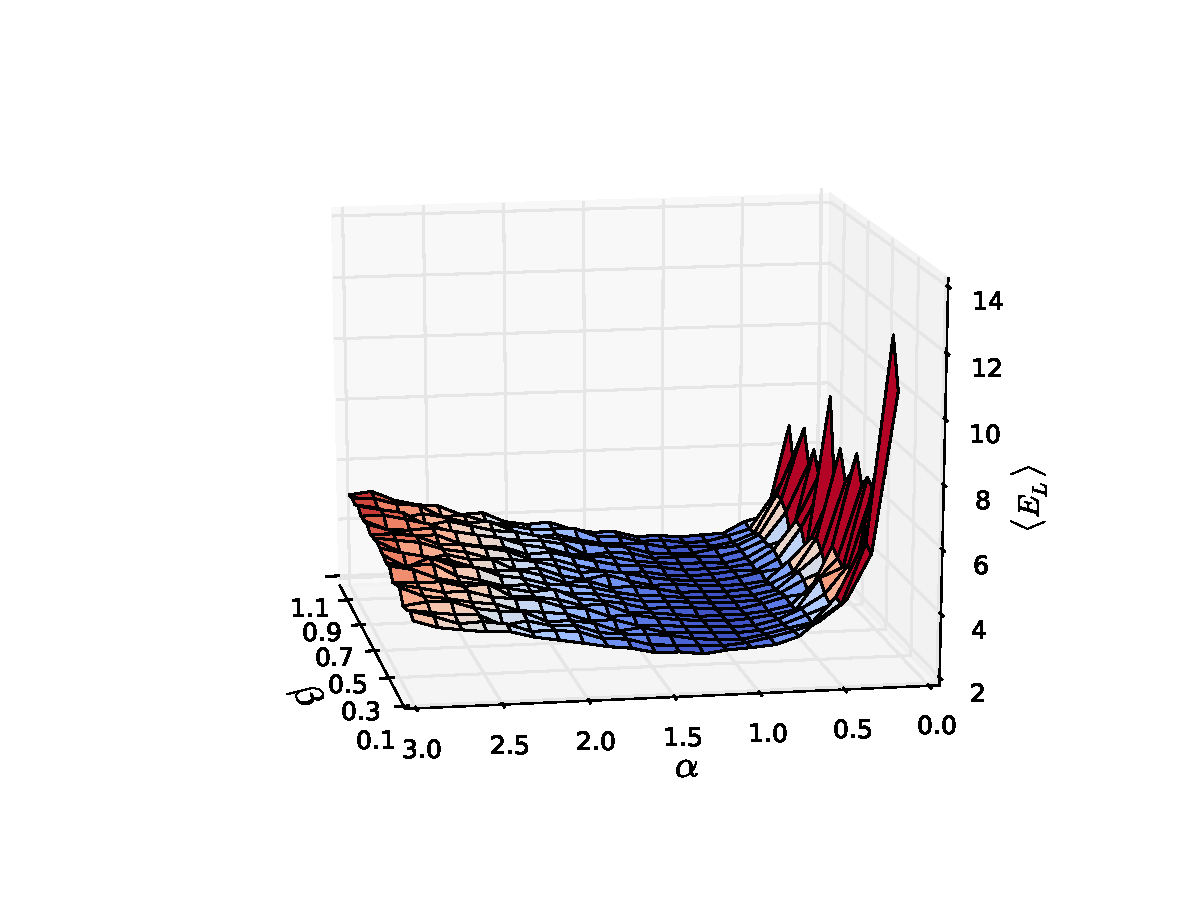
\includegraphics[width=0.8\linewidth, trim={0 2cm 0 4.5cm}, clip]{figures/energySurface/energyPlot15x15N2}
\caption{Local energy as a function of the parameters $\alpha$ and $\beta$ in the two-electron system.}
\label{fig:energyPlot15x15N2}
\end{figure}
	
	\subsection{Blocking method} \label{blockingTheory}
	
	After having run a Monte Carlo simulation, the variation in estimated local energies are calculated as
	\begin{equation}
		\sigma = \sqrt{\frac{1}{n}\lr{\langle E_L^2 \rangle - \langle E_L \rangle^2}}. \label{uncorelatedVariance}
	\end{equation} 
	However, these values will be much too low.
	This is because one assumes all data to be completely uncorrelated. Each energy is calculated by a small perturbation to the system setting\footnote{In the program discussed here, only a single dimension of a single particle will be moved each step.}, which means each new setting is very dependant on the previous setting. After sufficiently many perturbations, though, the system at step $i$ will be so different from that of step $j$, that $\langle E_L\rangle_i$ is basically uncorrelated to  $\langle E_L\rangle_j$, but not for all $\langle E_L\rangle_k$ between $i$ and $j$. Ideally, one would like to find a \emph{correlation time} $\tau$ such that $i$ and $j$ will be uncorrelated if a time greater than $\tau$ has passed. If $\Delta t$ is the time between two Metropolis steps, then one would like to find $|i-j|$ in $\tau = |i-j|\Delta t$.\\
	A method of dealing with this is the blocking technique. The set of $\langle E_L\rangle$ measurements is grouped into blocks, each of which will give an average of average local energies. Afterwards, one can calculate the variance of these averages of averages. If then the standard deviation (equation above) is plotted as a function of the number of blocks\footnote{Inversely proportional to the block size by $\text{\scriptsize block size} = \frac{\text{number of samples}}{\text{number of blocks}}$}, one can find the lowest number of blocks where the curve approaches a plateau. Then one can calculate $\tau$ and find the correlation time. The true standard deviation is then:
	
	\begin{equation}
		\sigma=\sqrt{\frac{1+2\tau/\Delta t}{n}\left(\langle \mathbf{M}^2\rangle-\langle \mathbf{M}\rangle^2\right)}
	\end{equation}
	
	\subsection{Benchmarking}
	While the flowchart seems nice and compact, there is quite a bit code that needs implementing and some benchmarks would be nice. The first is so check if the program reproduces the energy expected for non-interacting electrons in a harmonic oscillator potential. This means that if we remove the Coulomb potential and set $a_{ij} = 0$, then the problem is simply several non-interacting harmonic oscillators and we are left with a simple harmonic oscillator with energies given as
	\begin{equation}
	E_{n_x,n_y} = \hbar\omega\lr{n_x + n_y +1}.
	\end{equation}
	In figure \ref{fig: spinFig} these energies levels are shown. If sums of these values are reproduced, it means our Slater determinant expressions are correctly implemented.
		
		
		\begin{figure}[H]
			\begin{center}
				\begin{tikzpicture}
				\begin{scope}[xshift=0cm, yshift = 0cm]
				\draw (0,0) -- (1,0);
				\draw [arrow] (0.33,-0.3)--(0.33,0.3);
				\draw [arrow] (0.66,0.3)--(0.66,-0.3);
				\end{scope}	
				
				\foreach \i in {-1,1}{
					\begin{scope}[xshift=\i cm, yshift = 1cm]
					\draw (0,0) -- (1,0);
					\draw [arrow] (0.33,-0.3)--(0.33,0.3);
					\draw [arrow] (0.66,0.3)--(0.66,-0.3);
					\end{scope}	
				}
				\foreach \i in {-2,0,2}{
					\begin{scope}[xshift=\i cm, yshift = 2cm]
					\draw (0,0) -- (1,0);
					\draw [arrow] (0.33,-0.3)--(0.33,0.3);
					\draw [arrow] (0.66,0.3)--(0.66,-0.3);
					\end{scope}	
				}
				\foreach \i in {-3,-1,1,3}{
					\begin{scope}[xshift=\i cm, yshift = 3cm]
					\draw (0,0) -- (1,0);
					\draw [arrow] (0.33,-0.3)--(0.33,0.3);
					\draw [arrow] (0.66,0.3)--(0.66,-0.3);
					\end{scope}	
				}
				
				\node [draw=none] (N2)  at (6.5,0) {$\phantom{1}\hbar\omega$};
				\node [draw=none] (N6)  at (6.5,1) {$2\hbar\omega$};
				\node [draw=none] (N12) at (6.5,2) {$3\hbar\omega$};
				\node [draw=none] (N20) at (6.5,3) {$4\hbar\omega$};
				\draw [dotted, thick] (2,0) -- (N2);
				\draw [dotted, thick] (3,1) -- (N6);
				\draw [dotted, thick] (4,2) -- (N12);
				\draw [dotted, thick] (5,3) -- (N20);
				
				\end{tikzpicture}
			\end{center}
			\caption{Illustrative figure of spin configurations in the closed shell system.}
			\label{fig: spinFig}
		\end{figure}
	
	Another benchmark is to reproduce the results of our program for the two body quantum dot. This system was solved analytically, and thus would show that the many body program can reproduce analytical results for 2 particles. This means that the full problem (Coulomb interactions and Jastrow correlations) works, at least for the two body system.
	
	In order to know if our two-body script works, we can compare with the work of Taut\footnote{M. Taut, Phys. Rev. A 48, 3561 - 3566 (1993)}, where he calculated the analytical solution of two electrons in an external oscillator potential with Coulomb interactions. He found:
	
	
	
	
	\section{Results}
	
		\begin{table}[H]
			\begin{center}
				\caption{Expectation values of local energy, kinetic energy and potential energy for $N=\{2,6,12,20\}$ and oscillator frequencies $\omega = \{1.0,\:0.5,\:0.1,\:0.05,\:0.01\}$. $\sigma$ is the standard deviation of $\langle E_L\rangle$, found by blocking. $\alpha,\beta$ are the optimal parameters.}
				\begin{tabularx}{\textwidth}{@{}YYYYYYYY@{}}
					$N$	& $\omega$ & $\bk{E_L}$ & $\bk{E_K}$ & $\bk{E_P}$ & $\sigma$ & $\alpha$ & $\beta$\\
					\toprule
					2	&	1.00 & 3.0031 & 0.9017 & 2.1013 & 1.53360e-6 & 1.09975 & 0.29472 \\
					&	0.50 & 1.6611 & 0.4559 & 1.2052 & 2.10014e-7 & 1.00015 & 0.29972 \\
					&	0.10 & 0.4415 & 0.0964 & 0.3451 & 5.09917e-5 & 0.99534 & 0.16965 \\
					&	0.05 & 0.2722 & 0.0480 & 0.2242 & 1.04670e-6 & 0.99591 & 0.22695 \\
					&   0.01 & 0.0873 & 0.0107 & 0.0766 & 4.48831e-4 & 0.99777 & 0.19004 \\
					\midrule
					6   &	1.00 & 20.204 & 3.8059 & 16.398 & 1.43517e-3 & 1.00127 & 0.46939 \\
					&	0.50 & 11.821 & 1.7797 & 10.042 & 1.60940e-3 & 0.97611 & 0.32474 \\
					&	0.10 & 3.7466 & 0.2878 & 3.3077 & 2.22848e-3 & 0.99293 & 0.32392 \\
					&	0.05 & 2.4792 & 0.2165 & 2.2627 & 3.35813e-3 & 0.96891 & 0.37989 \\
					&   0.01 & 0.8972 & 0.0472 & 0.8500 & 1.84693e-3 & 1.00751 & 0.21825 \\
					\midrule
					12  &	1.00 & 65.776 & 8.7763 & 57.000 & 1.46457e-2 & 0.80173 & 0.80030 \\
					&	0.50 & 39.223 & 4.0024 & 35.221 & 1.03759e-2 & 0.80003 & 0.50039 \\
					&	0.10 & 14.683 & 1.1936 & 13.489 & 3.82364e-2 & 1.00071 & 0.69019 \\
					&	0.05 & 7.6569 & 0.4908 & 7.1661 & 6.69810e-3 & 0.94721 & 0.15057 \\
					&   0.01 & 3.2558 & 0.0937 & 3.1621 & 2.22688e-2 & 0.70992 & 0.34371 \\
					\midrule
					20  &	1.00 & 157.48 & 20.430 & 137.05 & 2.35715e-2 & 0.92930 & 0.80390 \\
					&	0.50 & 93.981 & 7.9372 & 86.044 & 1.42877e-2 & 0.82140 & 0.47966 \\
					&	0.10 & 30.157 & 1.1977 & 28.959 & 1.63797e-2 & 0.53094 & 0.39662 \\
					&	0.05 & 18.667 & 0.5123 & 18.155 & 1.45351e-2 & 0.43081 & 0.31274 \\
					&   0.01 & 6.2090 & 0.0821 & 6.1269 & 6.18577e-3 & 0.37267 & 0.12807 \\
					\bottomrule
				\end{tabularx}
				\label{tab:EnergiesVarianceAndOptimalParameters}
			\end{center}
		\end{table}
	
	%For the standard deviations ($\sigma$), the blocking plots were easily readable for $N=2$ and $N=6$, but the "plateau" for higher particle numbers were a bit hard to read. In figure \ref{fig:blocking}, there are two blocking plots presented. As can be seen, for $N=6$ the plateau starts at about 10000-15000, while for $N=20$ it is not completely clear. However, both were deemed to lie in the region 10000-15000 for these specific cases.
	
	
	% YO BROS. THIS SHOULD PROBABLY GO IN THE COMMENTS SECTION, BUT WHO CARES, RIGHT? YOU FIX IT! BTW, EMAUS.... I'M USING CAPS.
	In order to give a correct value of the standard deviation (in $\bk{E_L}$), which also considers the covariance, we used the method of blocking described in section \ref{blockingTheory}. A couple of the plots produced is shown in figure \ref{fig:blocking}. These plots show a trend in the behavior of the correlation length $\tau$. Comparing figures on the same row, we see that $\tau$ increases as $\omega$ decreases. Also, if we compare figures on the same column, we see that $\tau$ increases as $N$ increases.
	
	The reason why $\tau$ increases as $N$ increases is intuitively simple to understand. If we have a system of many particles, more particles will be stationary at each time step. It will have a higher degree of correlation than that of a system  of less particles. Thus, since we have to perform more moves in order to make a configuration that is basically uncorrelated with the initial, the correlation length is larger.
	The other behavior, that $\tau$ increases as $\omega$ decreases, is due to the fact that as $\omega$ decreases, the particles are free to move farther away from the origin, as can be observed in figure \ref{fig:OnebodyD}. Since the mean distance between electrons will increase as $\omega$ decreases, the relative change in the configuration due to a move will be smaller. Therefore we must perform more moves to reach an approximately uncorrelated configuration.                                                                                                                                                                                                                                                       
	
		\begin{figure}[H]
			
			\begin{subfigure}{0.5\textwidth}
				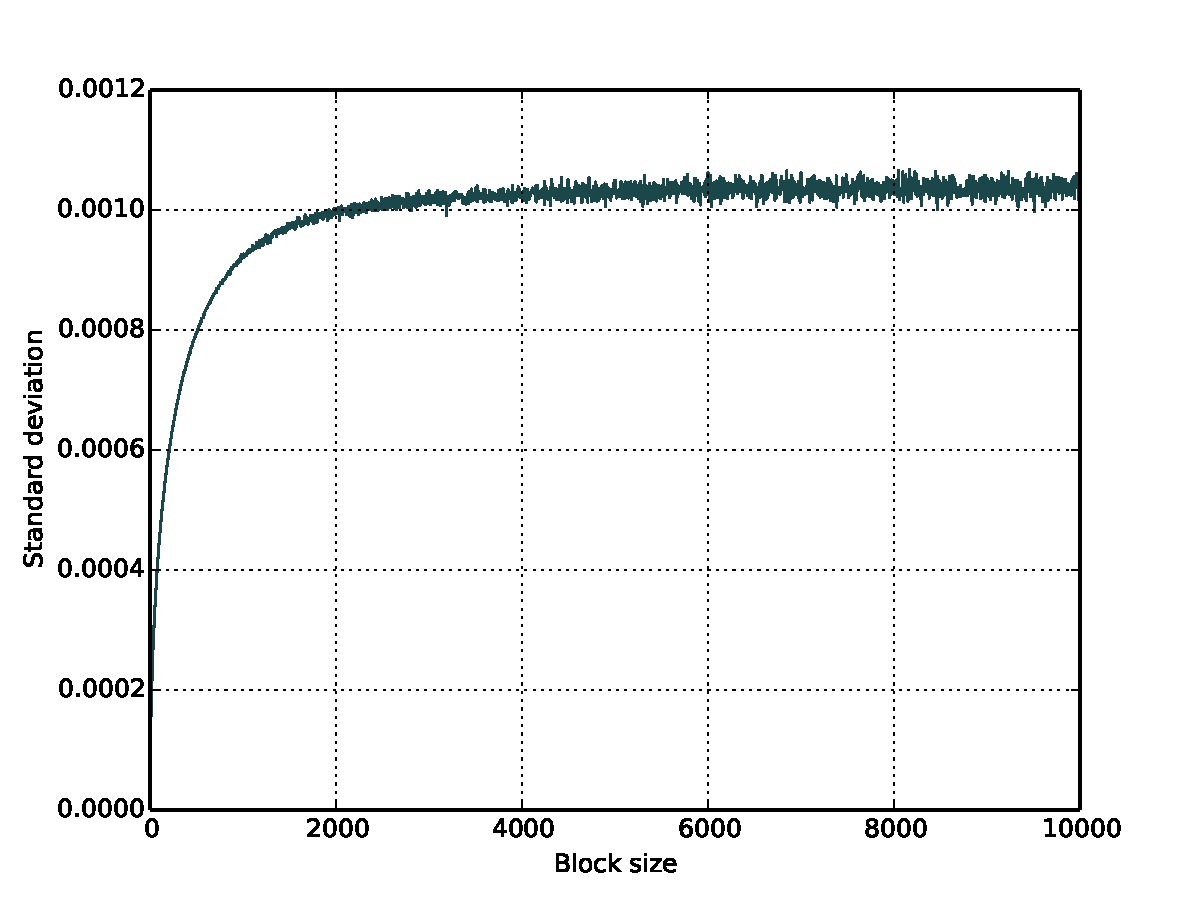
\includegraphics[scale=0.43]{figures/blocking/filipN2w100.pdf}
				\caption{$N=2,\:\omega=1.0$}
				\label{fig:blockingN2w100}
			\end{subfigure}
			\begin{subfigure}{0.5\textwidth}
				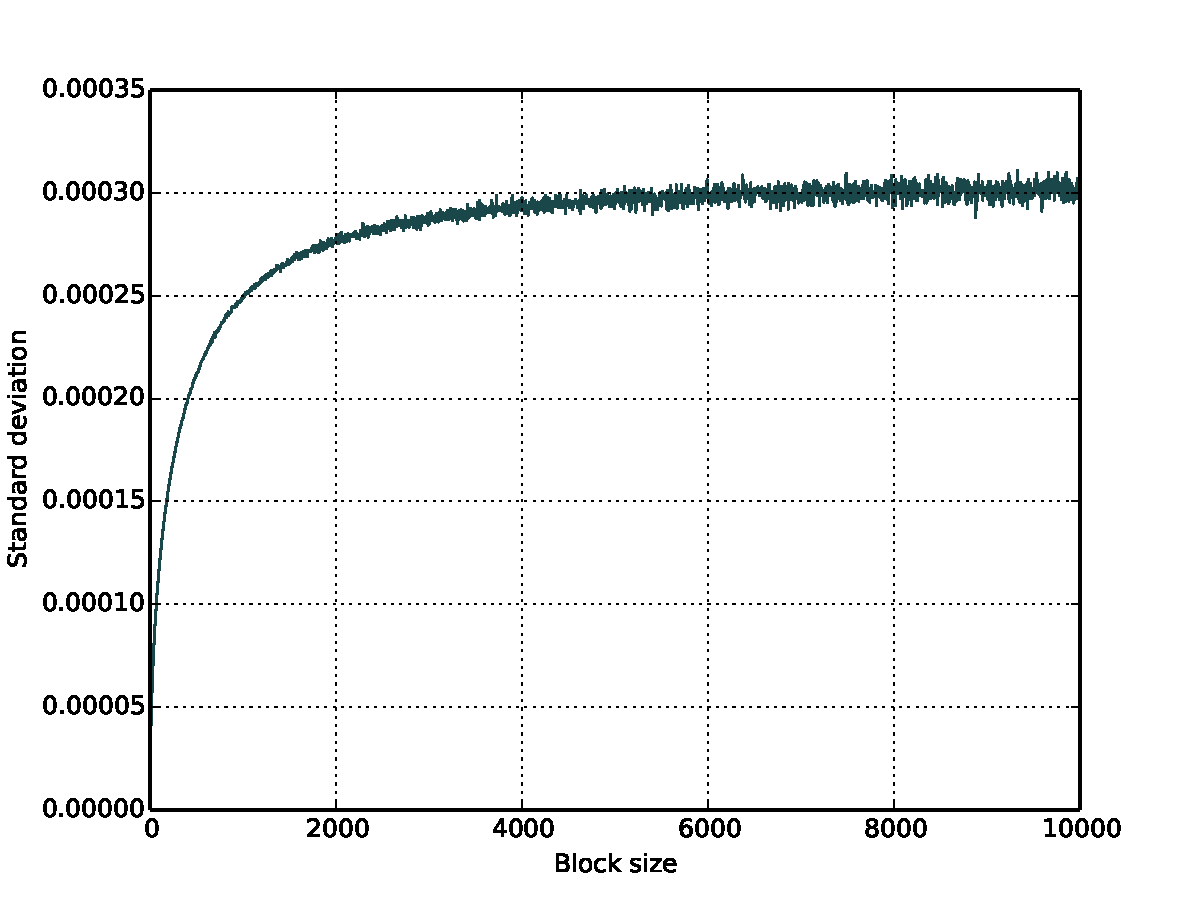
\includegraphics[scale=0.43]{figures/blocking/filipN2w50.pdf}
				\caption{$N=2,\:\omega=0.5$}
				\label{fig:blockingN2w50}
			\end{subfigure}
			
			\vspace{1mm}
			
			\begin{subfigure}{0.5\textwidth}
				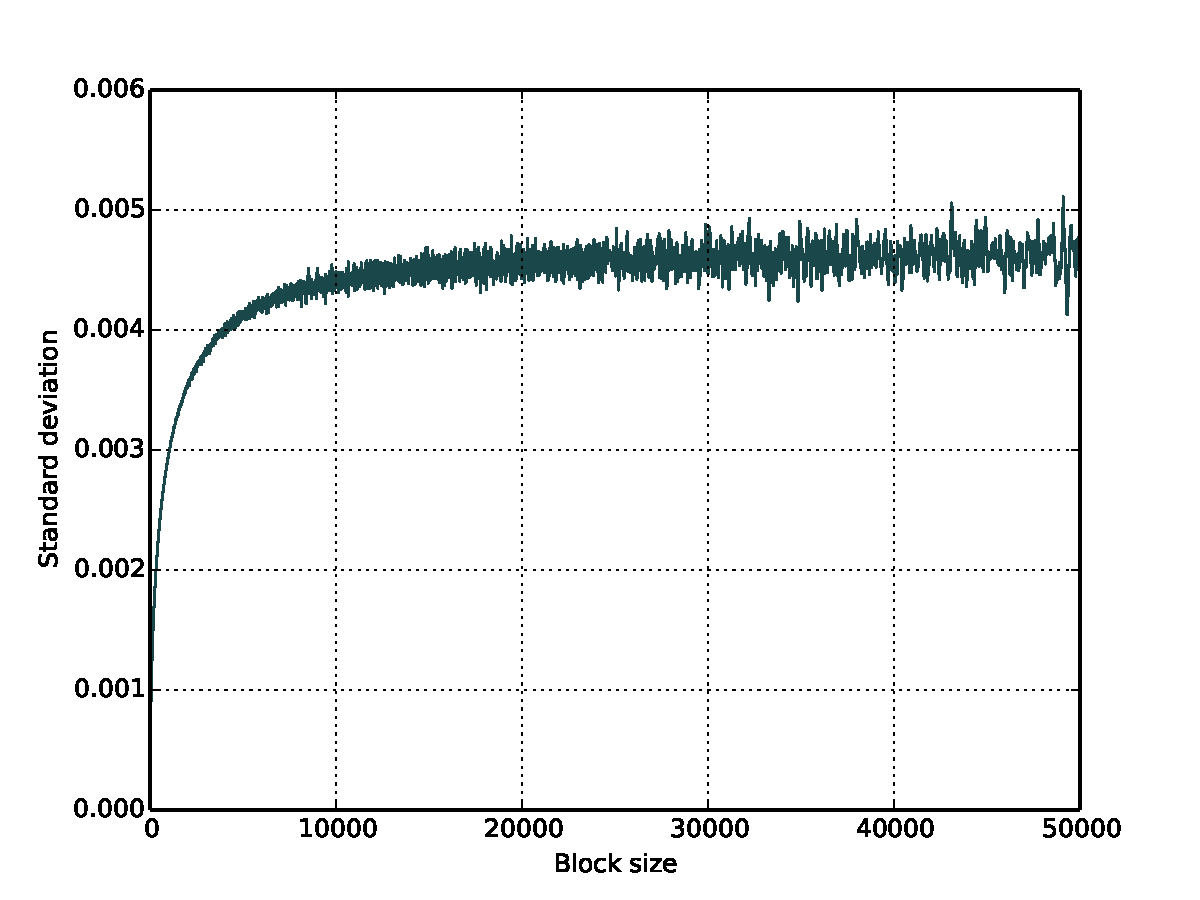
\includegraphics[scale=0.43]{figures/blocking/filipN6w100.pdf}
				\caption{$N=6,\:\omega=1.0$}
				\label{fig:blockingN6w100}
			\end{subfigure}
			\begin{subfigure}{0.5\textwidth}
				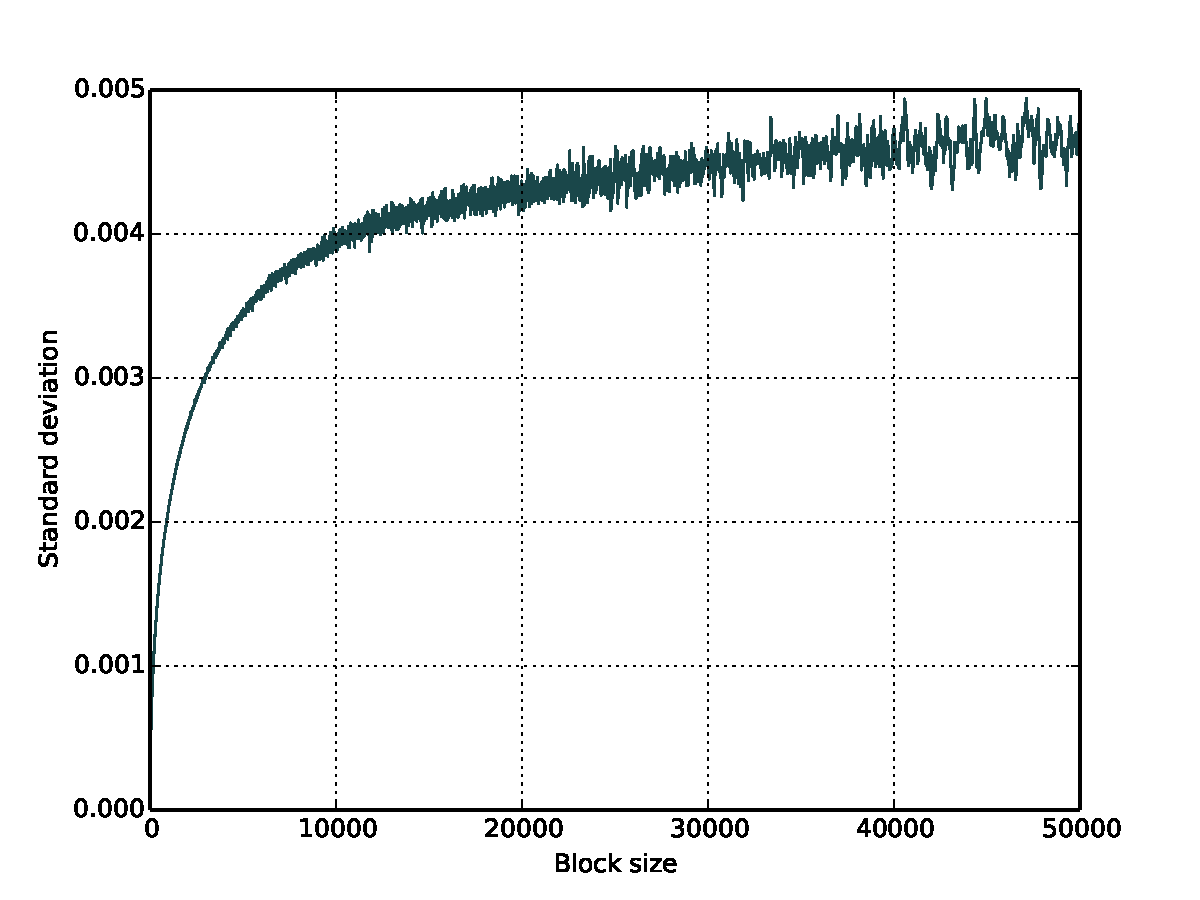
\includegraphics[scale=0.43]{figures/blocking/filipN6w50.pdf}
				\caption{$N=6,\:\omega=0.5$}
				\label{fig:blockingN6w50}
			\end{subfigure}
					
			\caption{Plots produced by the blocking method for systems of $N=\{2,6\}$ and $\omega=\{1, 0.5\} $.}
			\label{fig:blocking}
		\end{figure}
	
	\begin{table}[H]
		\begin{center}
			\caption{Local energy computed for systems without the Jastrow factor and Coulomb potential. This resembles a pure harmonic oscillator and the results are dead on.}
			\begin{tabularx}{0.5\textwidth}{@{}YYY@{}}
				\toprule
				$N$& $E_L$& $\sigma$ \\*
				\midrule
				2  & 2  & 0 \\
				6  & 10 & 0 \\
				12 & 28 & 0 \\
				20 & 60 & 0 \\
				\bottomrule
			\end{tabularx}
			\label{tab:HO}
		\end{center}
	\end{table}
	This matches the sums of the energy levels shown in figure \ref{fig: spinFig}, and infer that our Slater determinant expressions are implemented correctly.\\
	
	In table \ref{tab:varousOmega}, the energies for the two body system are presented, and was calculated using the analytical expressions from section 2.2. As is known, the energy for $\omega = 1.0$ and $N=2$ is exactly 3, and the table confirms this to quite a high accuracy.\\
	The average distance between the electrons for $\omega = 1.0$ is found to be $\langle r_{12}\rangle = 1.8$.
	
	\begin{table}[H]
		\begin{center}
			\caption{Expectation value of the kinetic energy and potential energy for several values of $\omega$.}
			\begin{tabularx}{0.5\textwidth}{@{}YYYY@{}}
				\toprule
				$\omega$& $\bk{E_K}$& $\bk{E_P}$ & $\bk{E_L}$ \\*
				\midrule
				0.01 & 0.0122 & 0.0969 & 0.0863\\
				0.05 & 0.0511 & 0.2274 & 0.2769\\
				0.1  & 0.0939 & 0.3544 & 0.4593\\
				1.0  & 0.8983 & 2.1475 & 3.0002\\
				\bottomrule
			\end{tabularx}
			\label{tab:varousOmega}
		\end{center}
	\end{table}
	
	Note, however, that each of the values listed in table \ref{tab:varousOmega} are from individual runs.
	The expectation values of the kinetic, potential and total (local) energy are thus not from the same simulation, and their value might not add up perfectly as $E_L = E_K + E_P$.
	The total energy is only shown to give a sense of its magnitude.
	
	\begin{figure}[H]
		
		\begin{subfigure}{0.5\textwidth}
			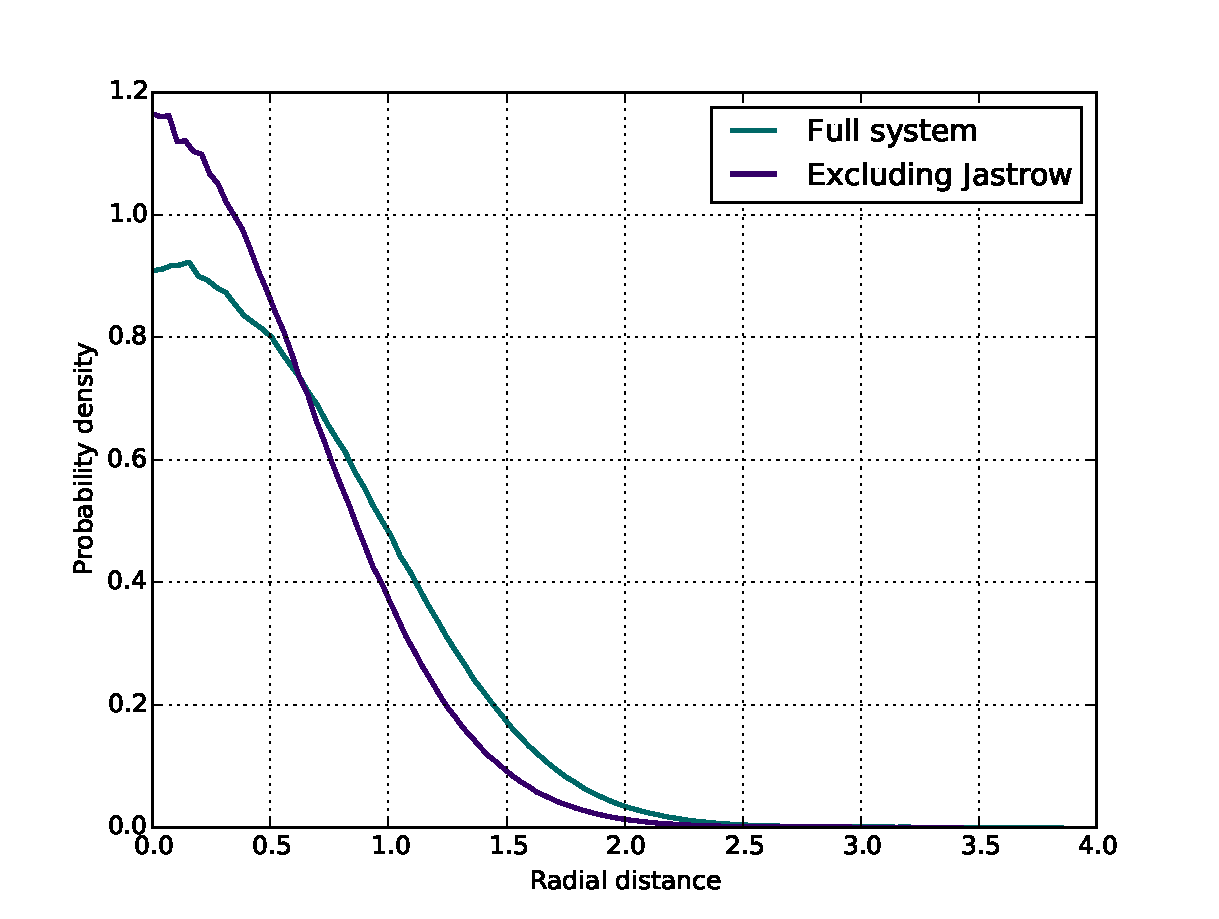
\includegraphics[width=\textwidth, height= 5cm]{figures/radialDistribution/OneBodyDensityN2w100Se7.pdf}
			\caption{$N=2,\:\omega=1.0$}
		\end{subfigure}
		\begin{subfigure}{0.5\textwidth}
			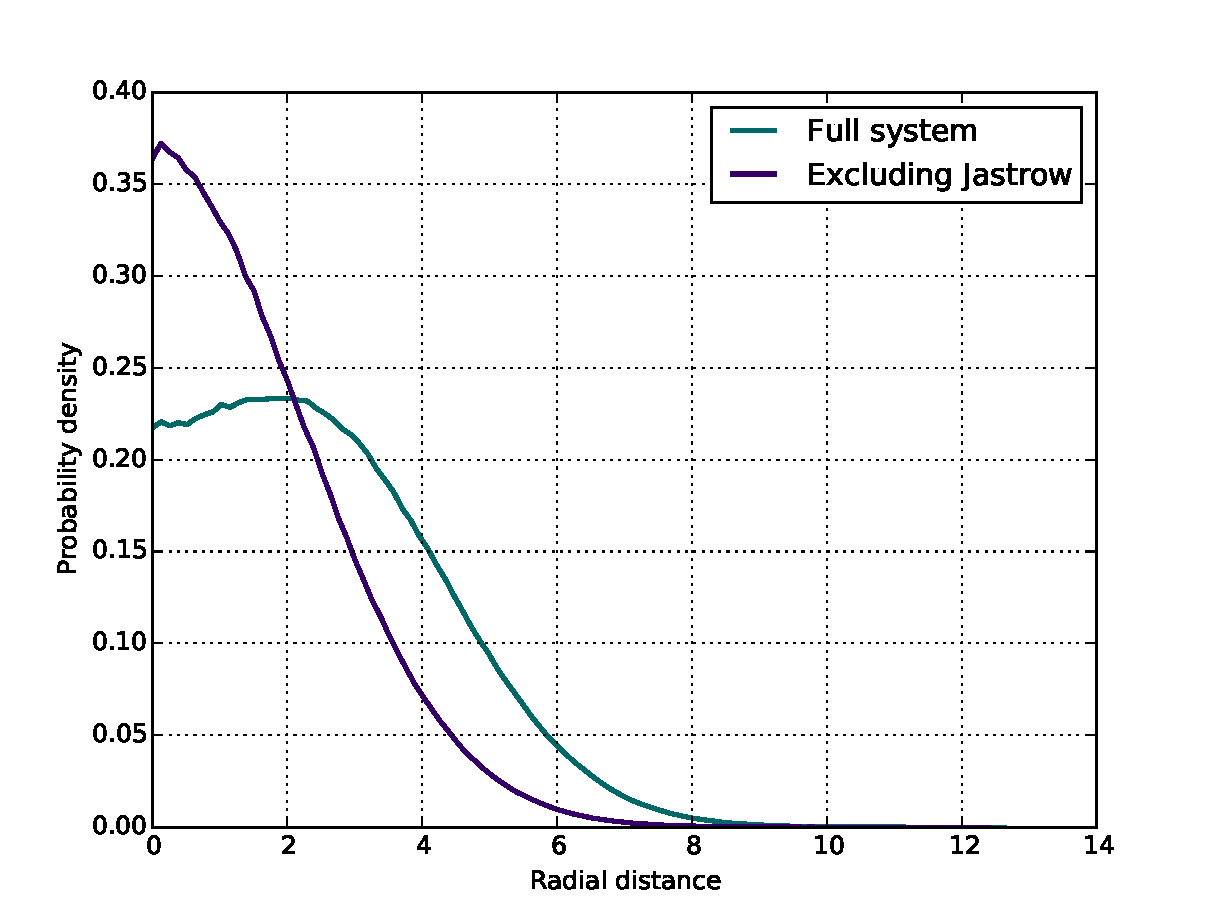
\includegraphics[width=\textwidth, height= 5cm]{figures/radialDistribution/OneBodyDensityN2w10Se7.pdf}
			\caption{$N=2,\:\omega=0.1$}
		\end{subfigure}
		
		\vspace{1mm}
		
		\begin{subfigure}{0.5\textwidth}
			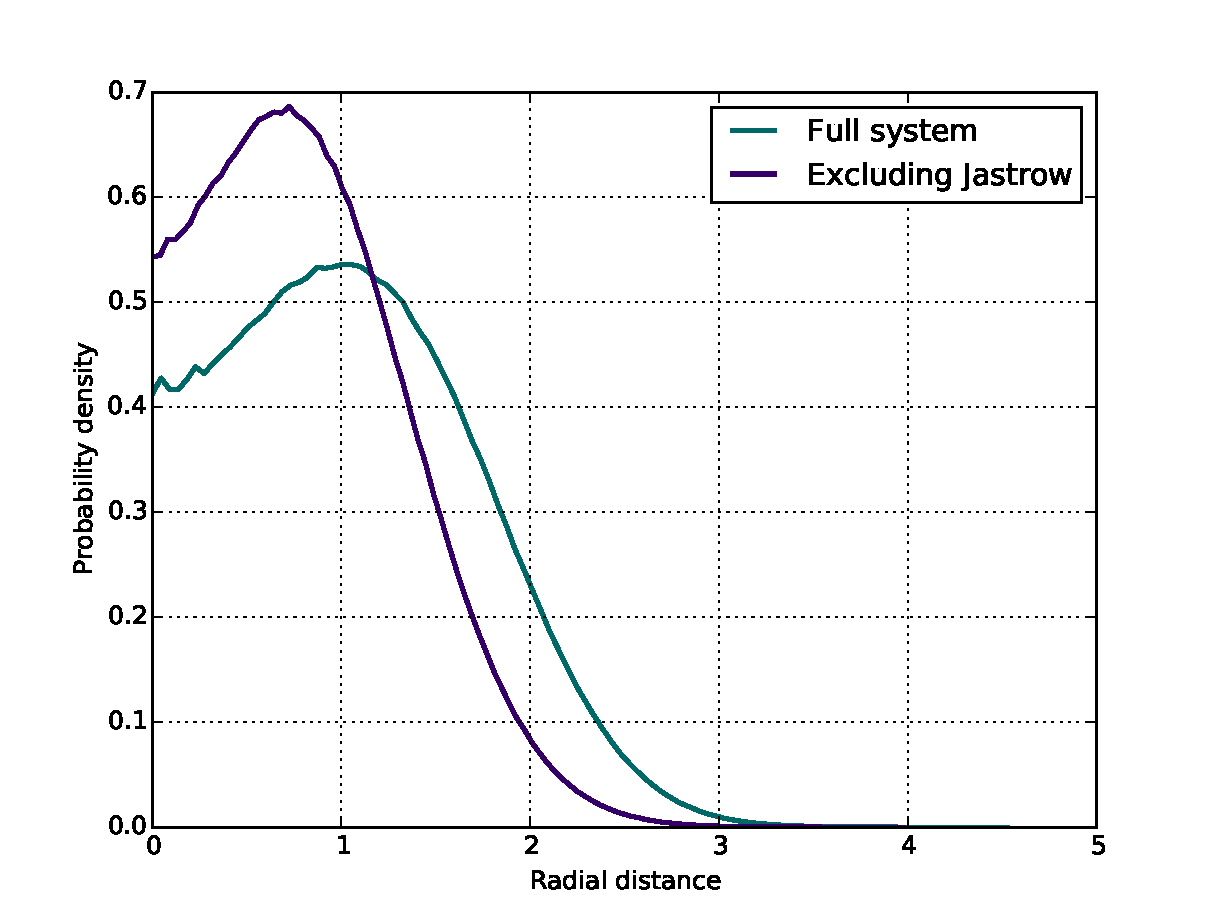
\includegraphics[width=\textwidth, height= 5cm]{figures/radialDistribution/OneBodyDensityN6w100Se7.pdf}
			\caption{$N=6,\:\omega=1.0$}
		\end{subfigure}
		\begin{subfigure}{0.5\textwidth}
			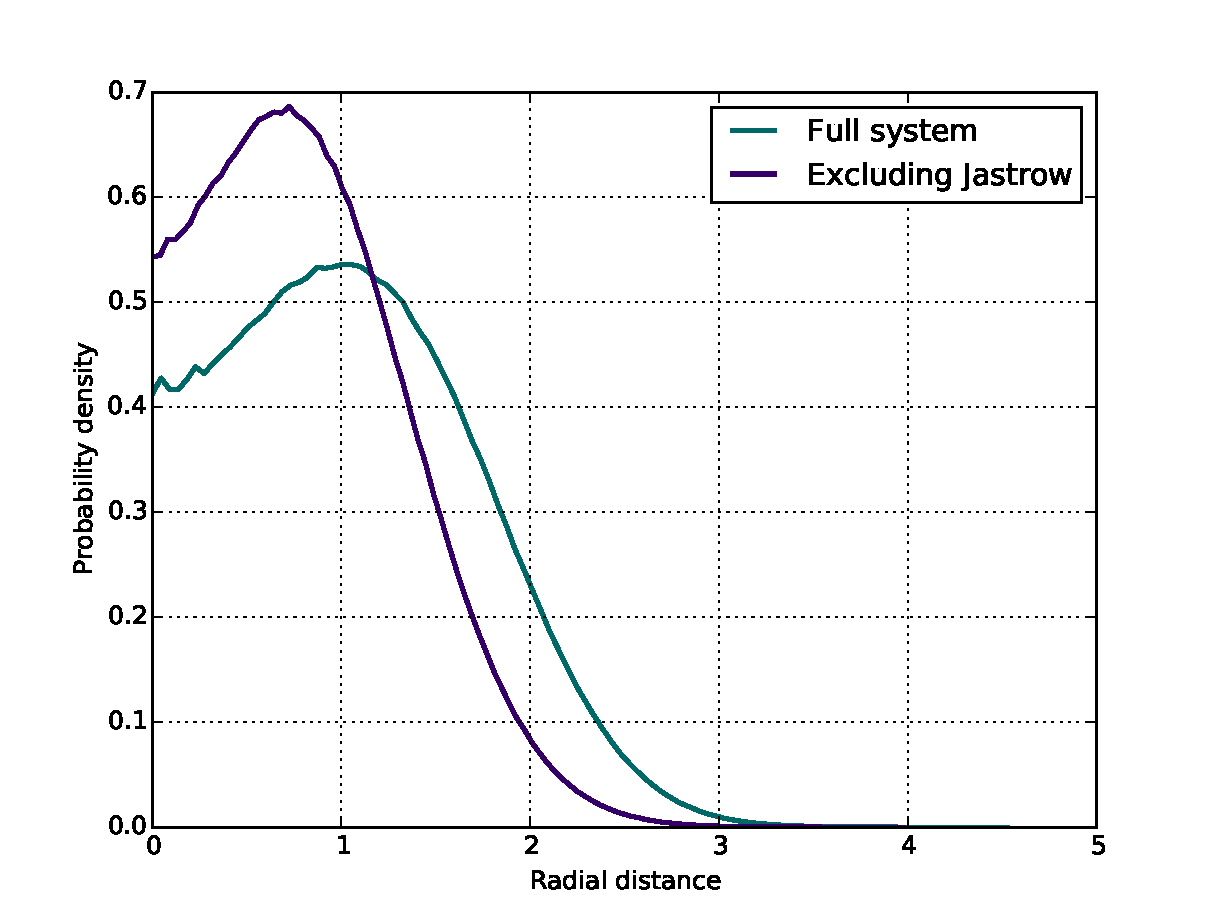
\includegraphics[width=\textwidth, height= 5cm]{figures/radialDistribution/OneBodyDensityN6w100Se7.pdf}
			\caption{$N=6,\:\omega=0.1$}
		\end{subfigure}
		
		\vspace{1mm}
		
		\begin{subfigure}{0.5\textwidth}
			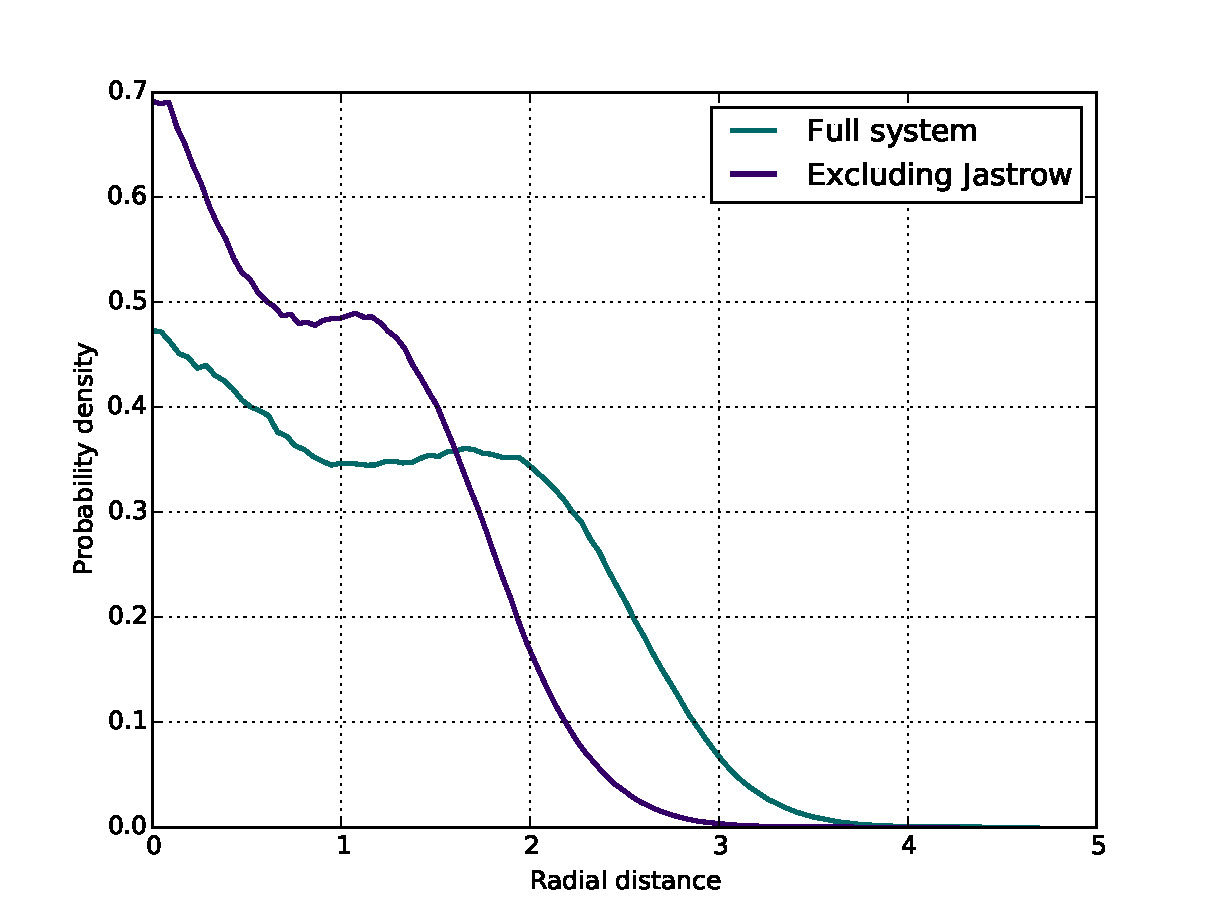
\includegraphics[width=\textwidth, height=5cm]{figures/radialDistribution/OneBodyDensityN12w100Se7.pdf}
			\caption{$N=12,\:\omega=1.0$}
		\end{subfigure}
		\begin{subfigure}{0.5\textwidth}
			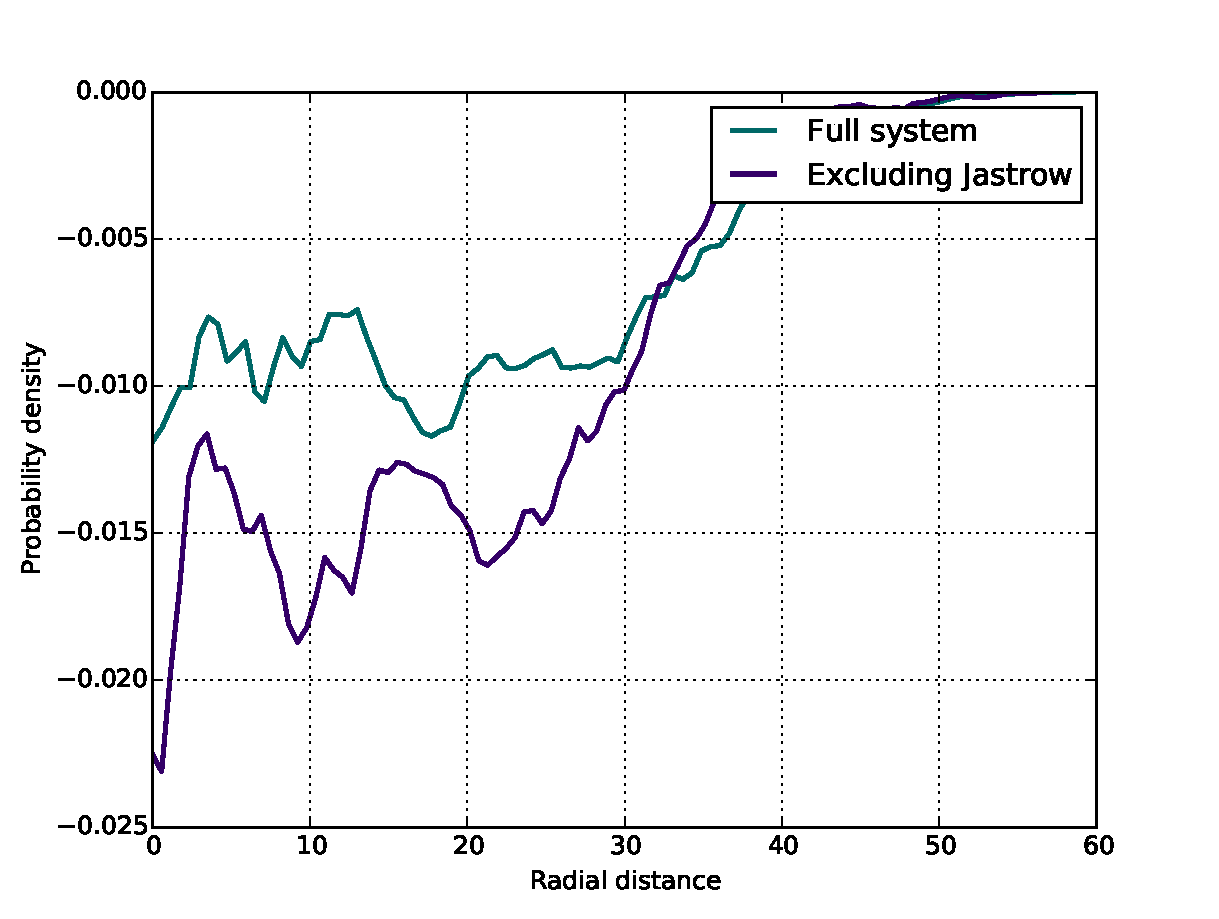
\includegraphics[width=\textwidth, height= 5cm]{figures/radialDistribution/OneBodyDensityN12w10Se7.pdf}
			\caption{$N=12,\:\omega=0.1$}
		\end{subfigure}
		
		\vspace{1mm}
		
		\begin{subfigure}{0.5\textwidth}
			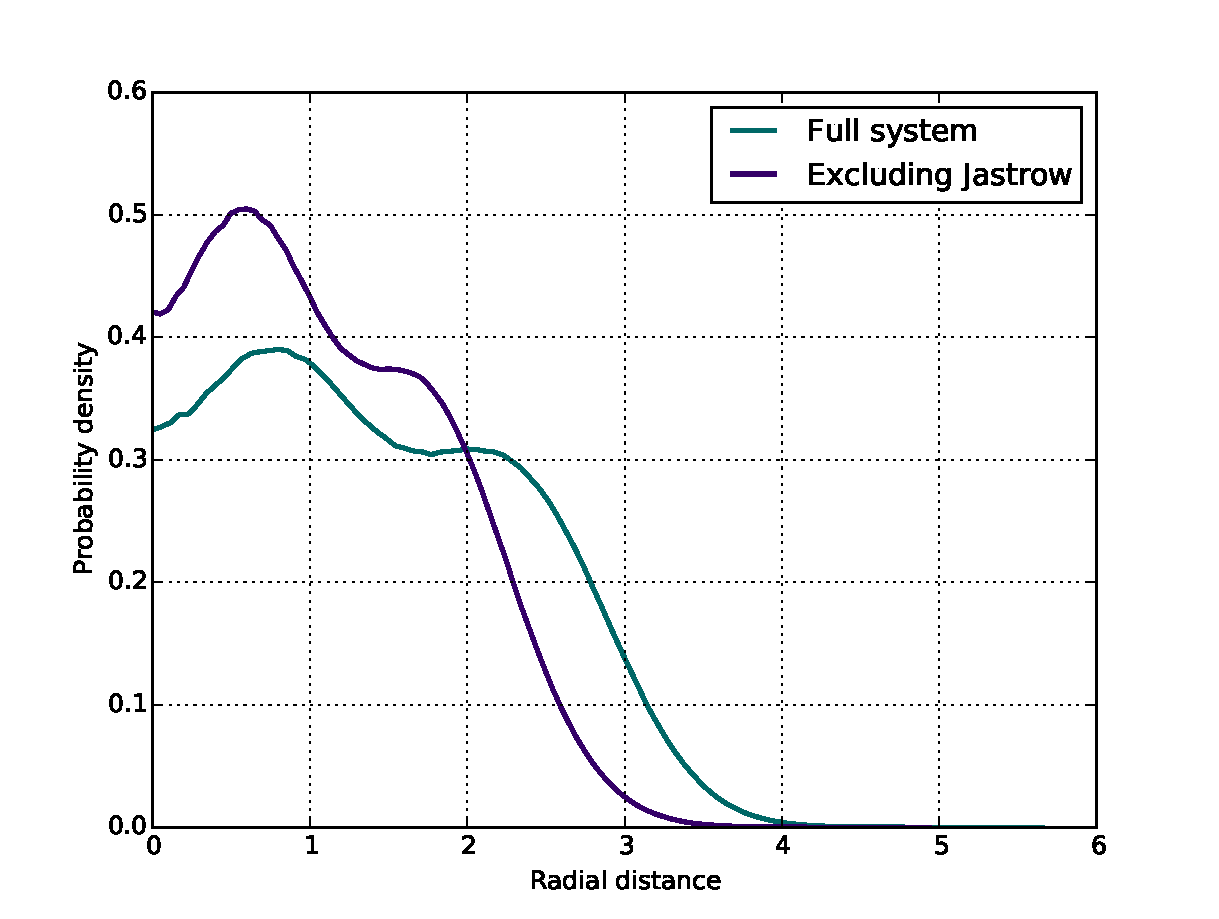
\includegraphics[width=\textwidth, height= 5cm]{figures/radialDistribution/OneBodyDensityN20w100Se8.pdf}
			\caption{$N=20,\:\omega=1.0$}
		\end{subfigure}
		\begin{subfigure}{0.5\textwidth}
			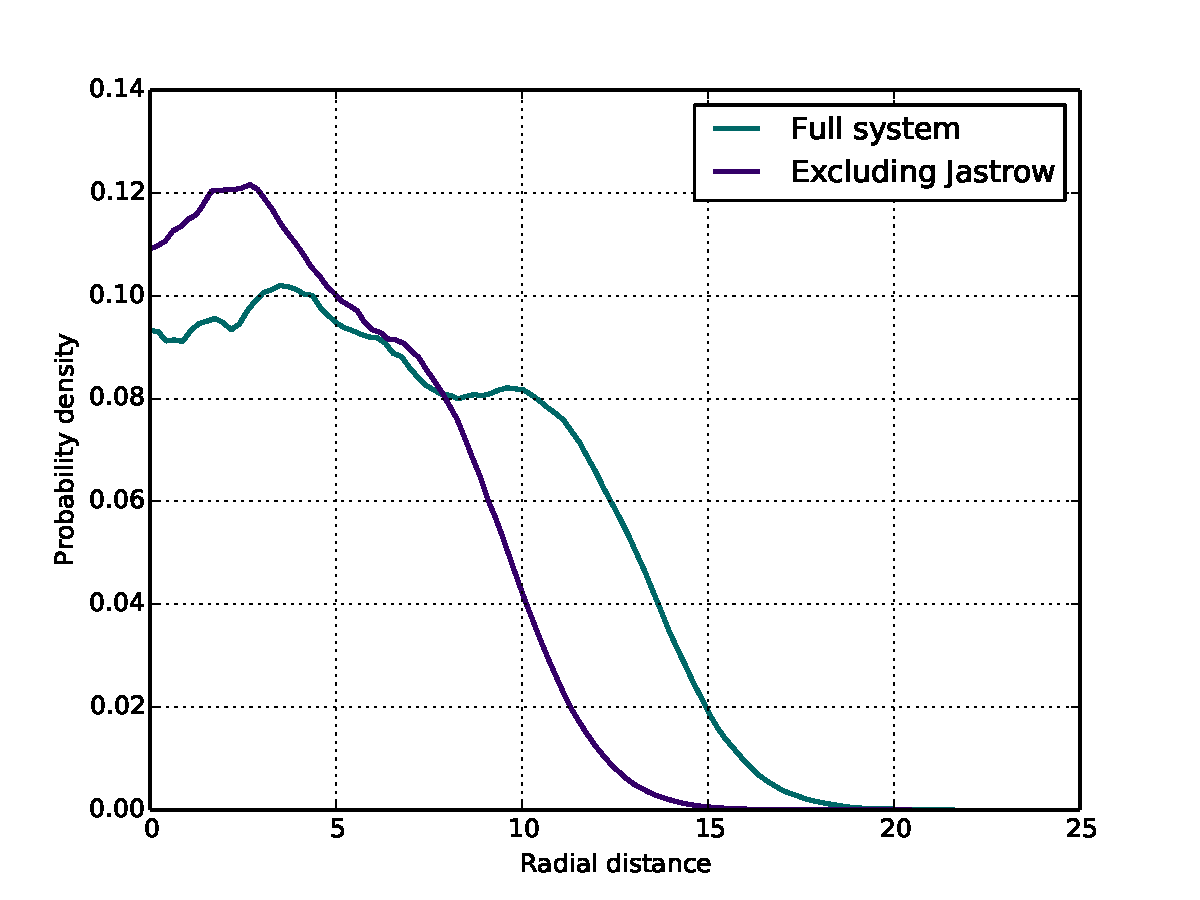
\includegraphics[width=\textwidth, height= 5cm]{figures/radialDistribution/OneBodyDensityN20w10Se8.pdf}
			\caption{$N=20,\:\omega=0.1$}
		\end{subfigure}
				
		\vspace{3mm}
				
		\caption{One-body densities (left) and radial distributions (right) for $N=\{2,6,12,20\}$ and $\omega = 1.0$.}
		\label{fig:Onebody}
	\end{figure}
	
	\newpage














\begin{figure}[H]
	
	\begin{subfigure}{0.5\textwidth}
		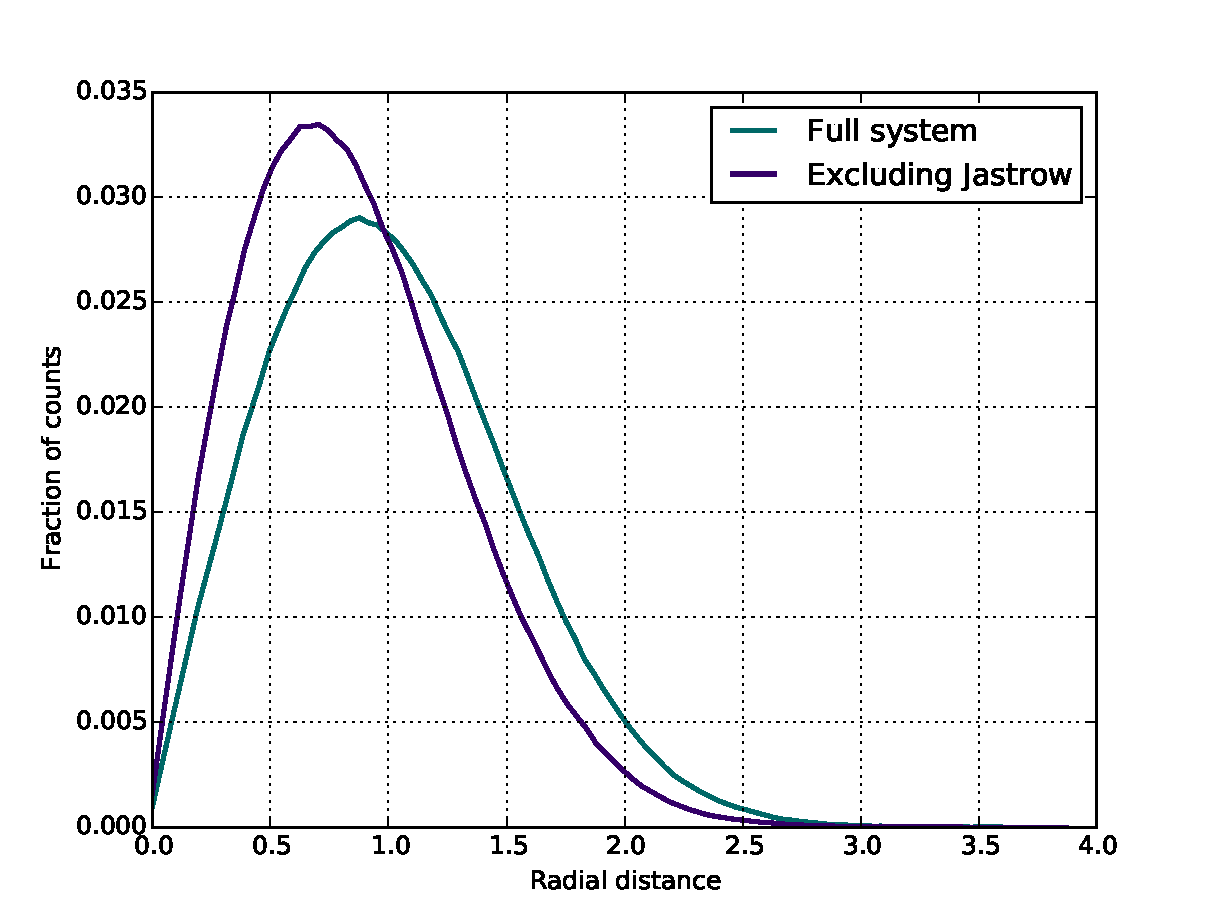
\includegraphics[width=\textwidth, height= 5cm]{figures/radialDistribution/radialDistributionN2w100Se7.pdf}
		\caption{$N=2,\:\omega=1.0$}
	\end{subfigure}
	\begin{subfigure}{0.5\textwidth}
		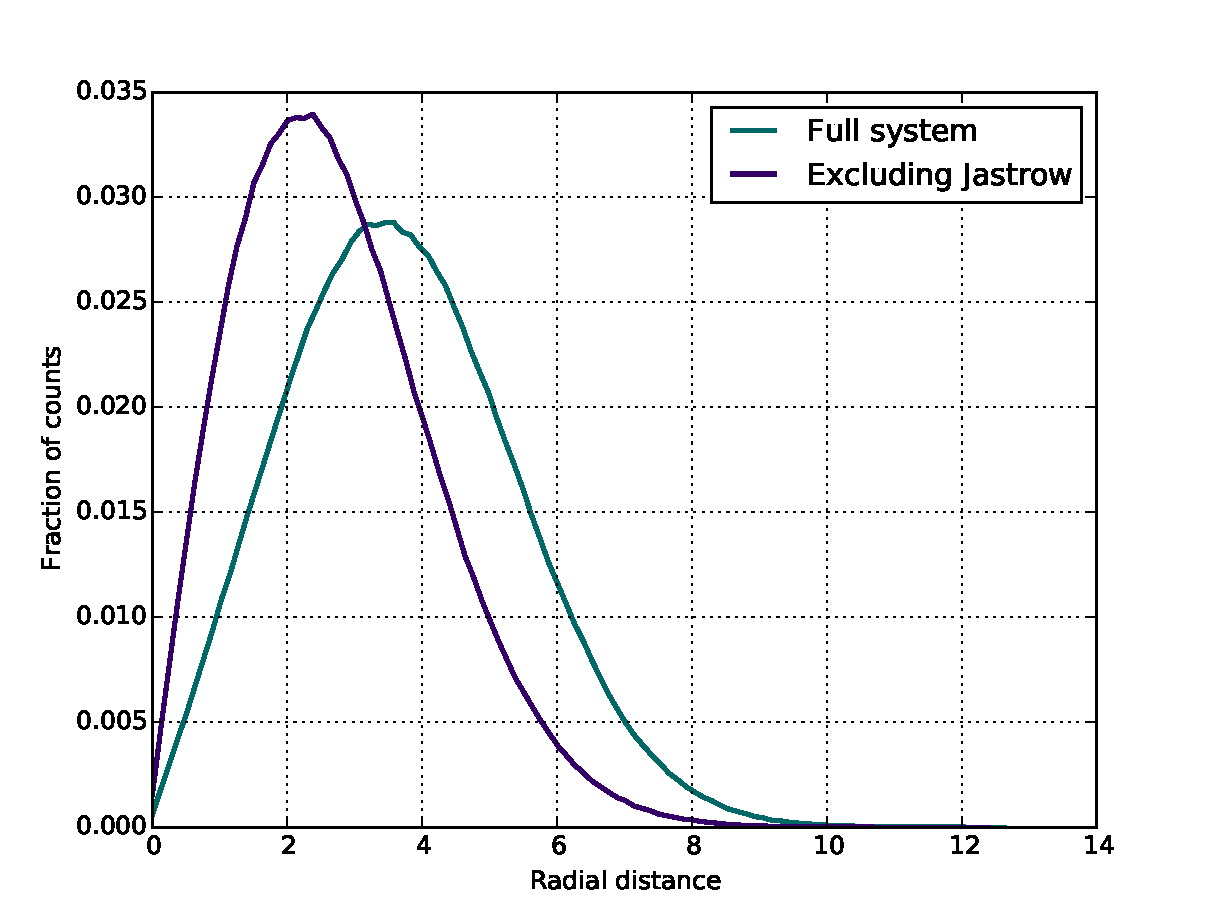
\includegraphics[width=\textwidth, height= 5cm]{figures/radialDistribution/radialDistributionN2w10Se7.pdf}
		\caption{$N=2,\:\omega=0.1$}
	\end{subfigure}
	
	\vspace{1mm}
	
	\begin{subfigure}{0.5\textwidth}
		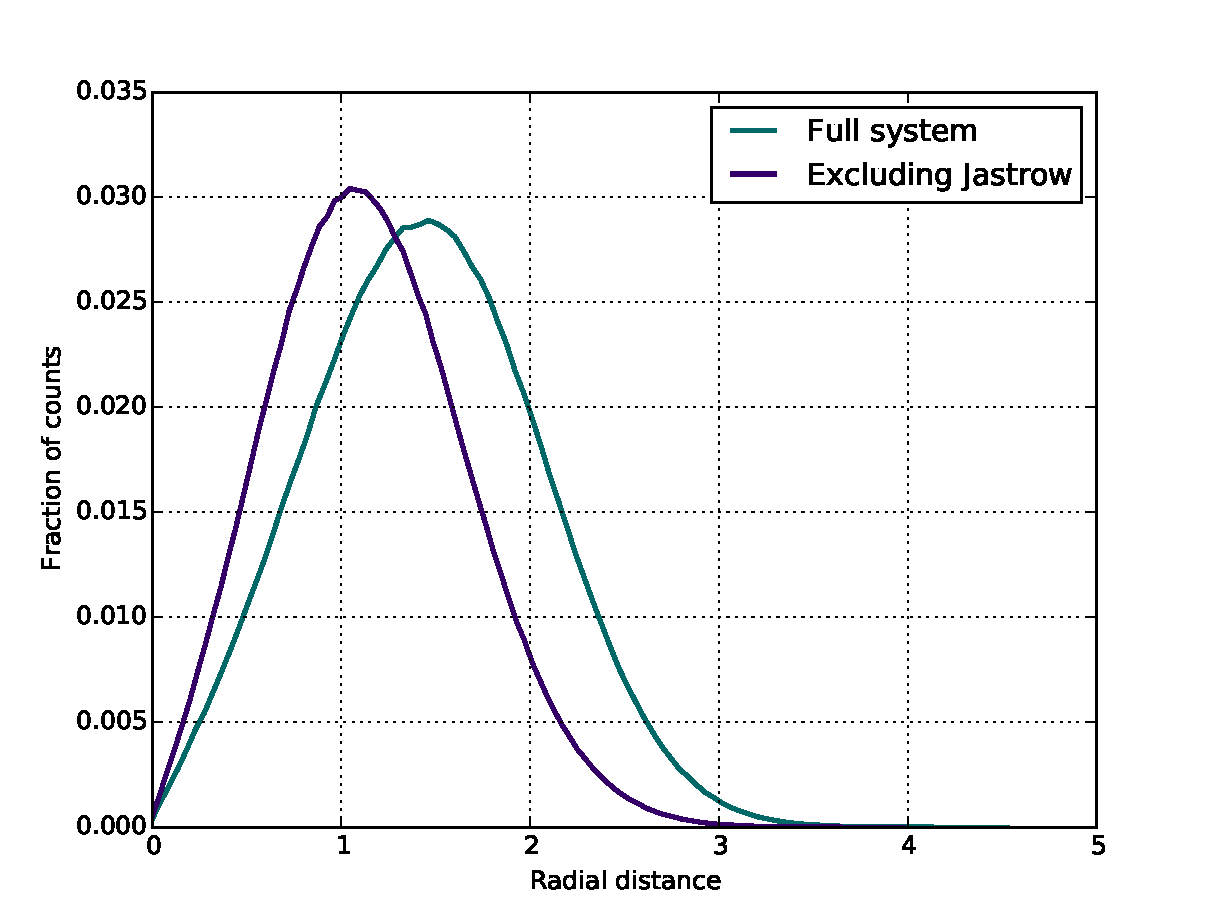
\includegraphics[width=\textwidth, height= 5cm]{figures/radialDistribution/radialDistributionN6w100Se7.pdf}
		\caption{$N=6,\:\omega=1.0$}
	\end{subfigure}
	\begin{subfigure}{0.5\textwidth}
		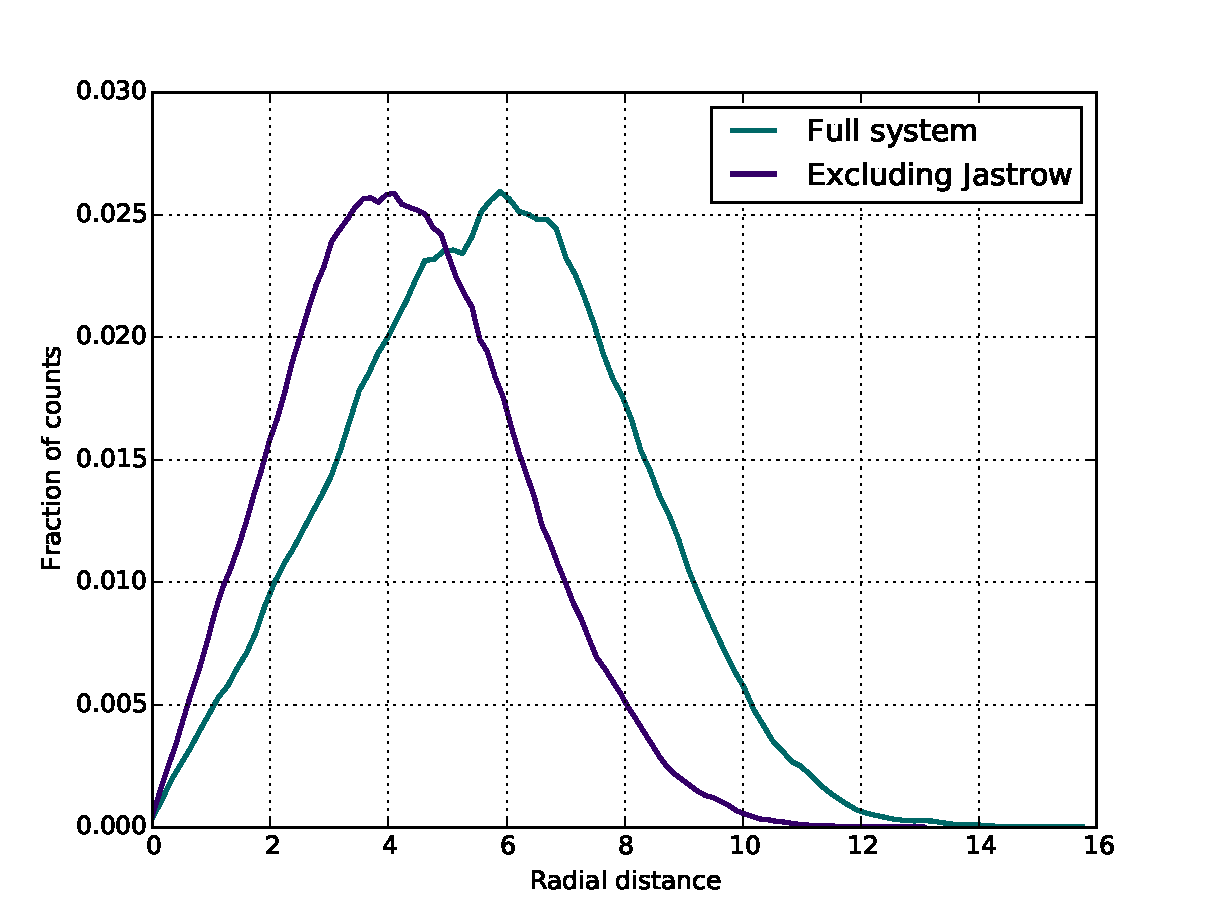
\includegraphics[width=\textwidth, height= 5cm]{figures/radialDistribution/radialDistributionN6w10Se7.pdf}
		\caption{$N=6,\:\omega=0.1$}
	\end{subfigure}
	
	\vspace{1mm}
	
	\begin{subfigure}{0.5\textwidth}
		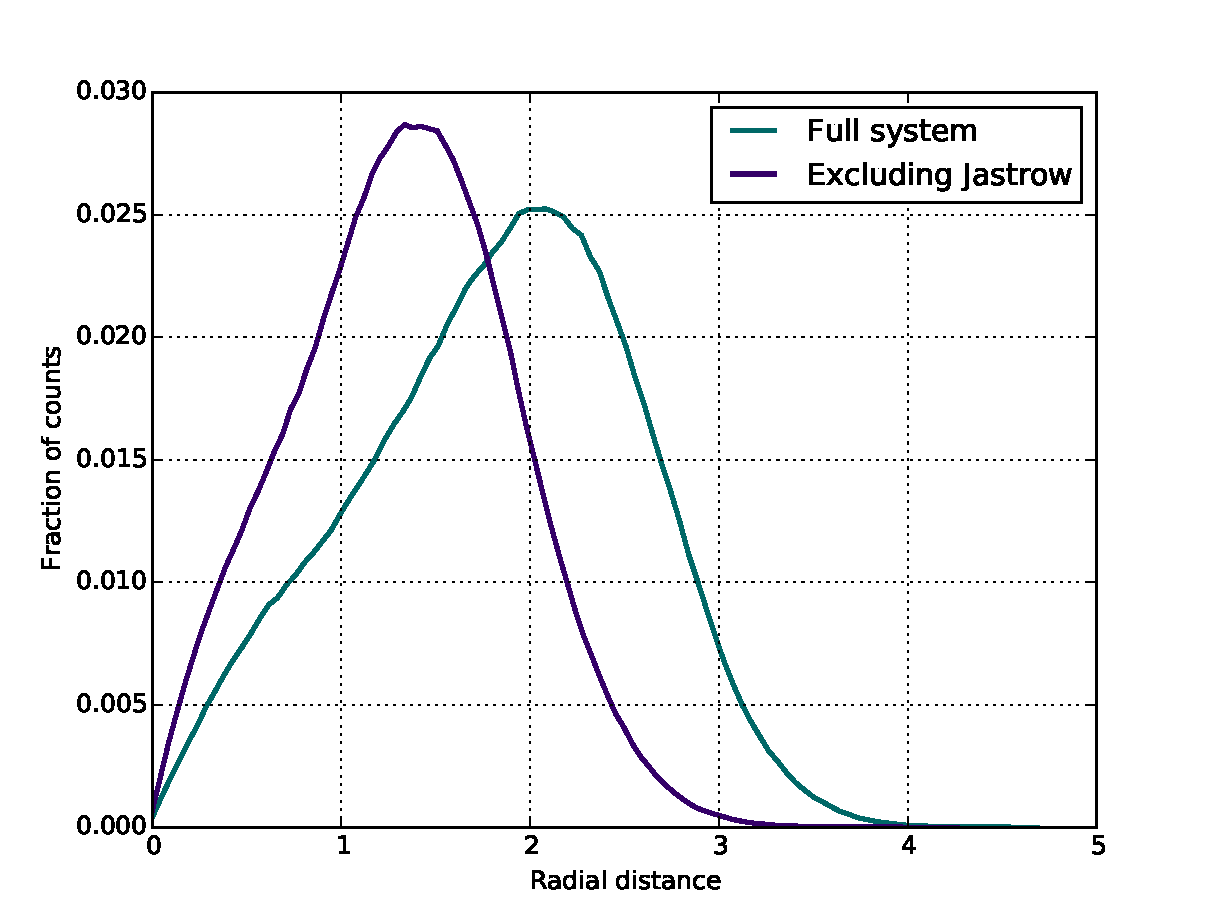
\includegraphics[width=\textwidth, height=5cm]{figures/radialDistribution/radialDistributionN12w100Se7.pdf}
		\caption{$N=12,\:\omega=1.0$}
	\end{subfigure}
	\begin{subfigure}{0.5\textwidth}
		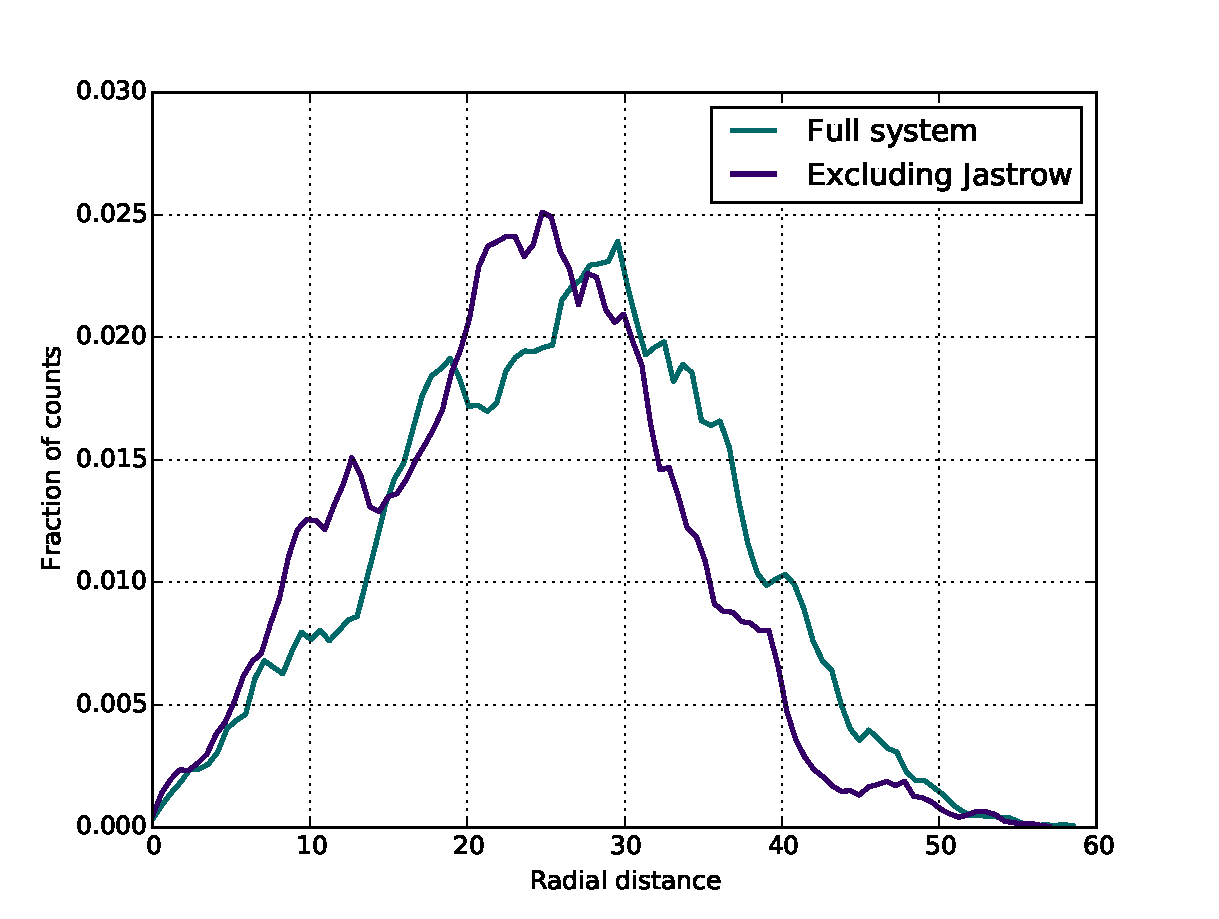
\includegraphics[width=\textwidth, height= 5cm]{figures/radialDistribution/radialDistributionN12w10Se7.pdf}
		\caption{$N=12,\:\omega=0.1$}
	\end{subfigure}
	
	\vspace{1mm}
	
	\begin{subfigure}{0.5\textwidth}
		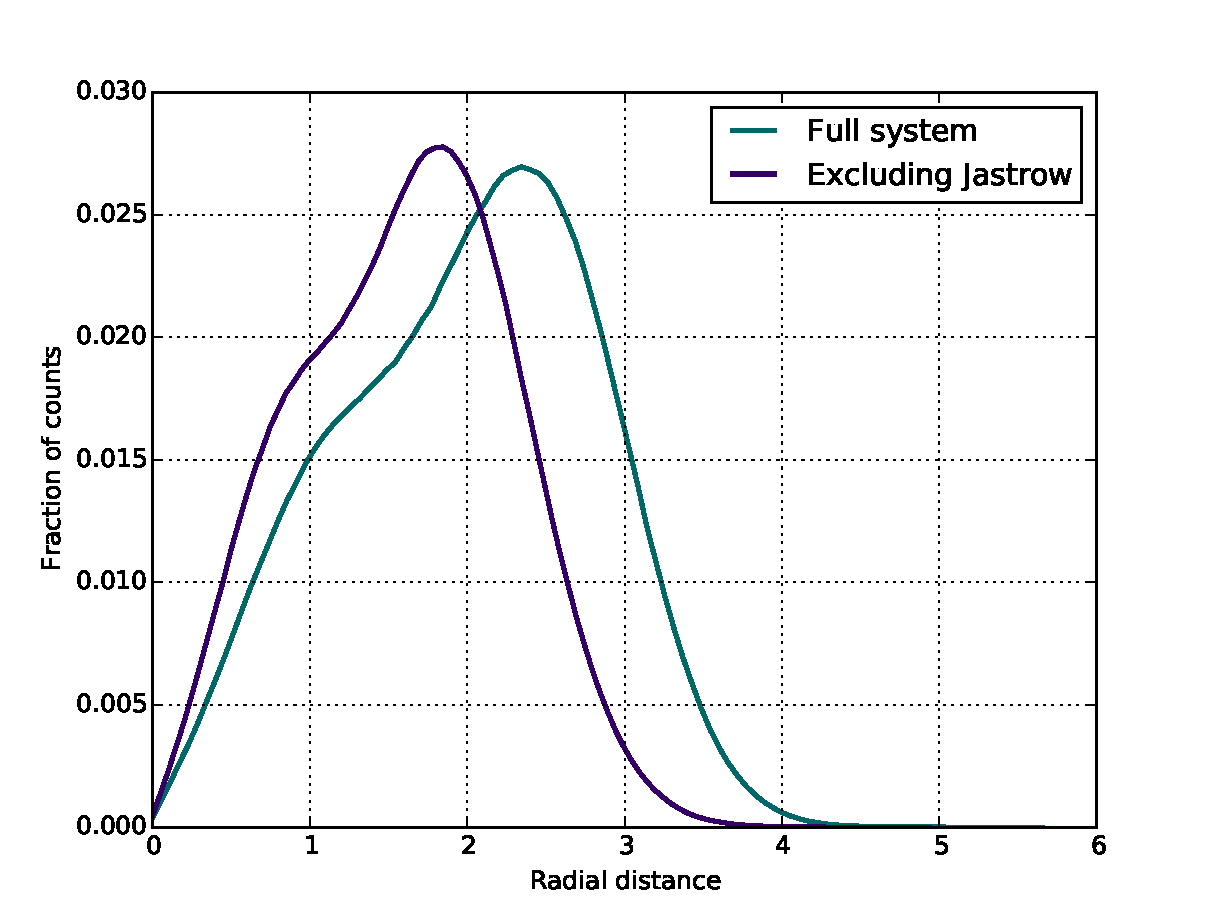
\includegraphics[width=\textwidth, height= 5cm]{figures/radialDistribution/radialDistributionN20w100Se8.pdf}
		\caption{$N=20,\:\omega=1.0$}
	\end{subfigure}
	\begin{subfigure}{0.5\textwidth}
		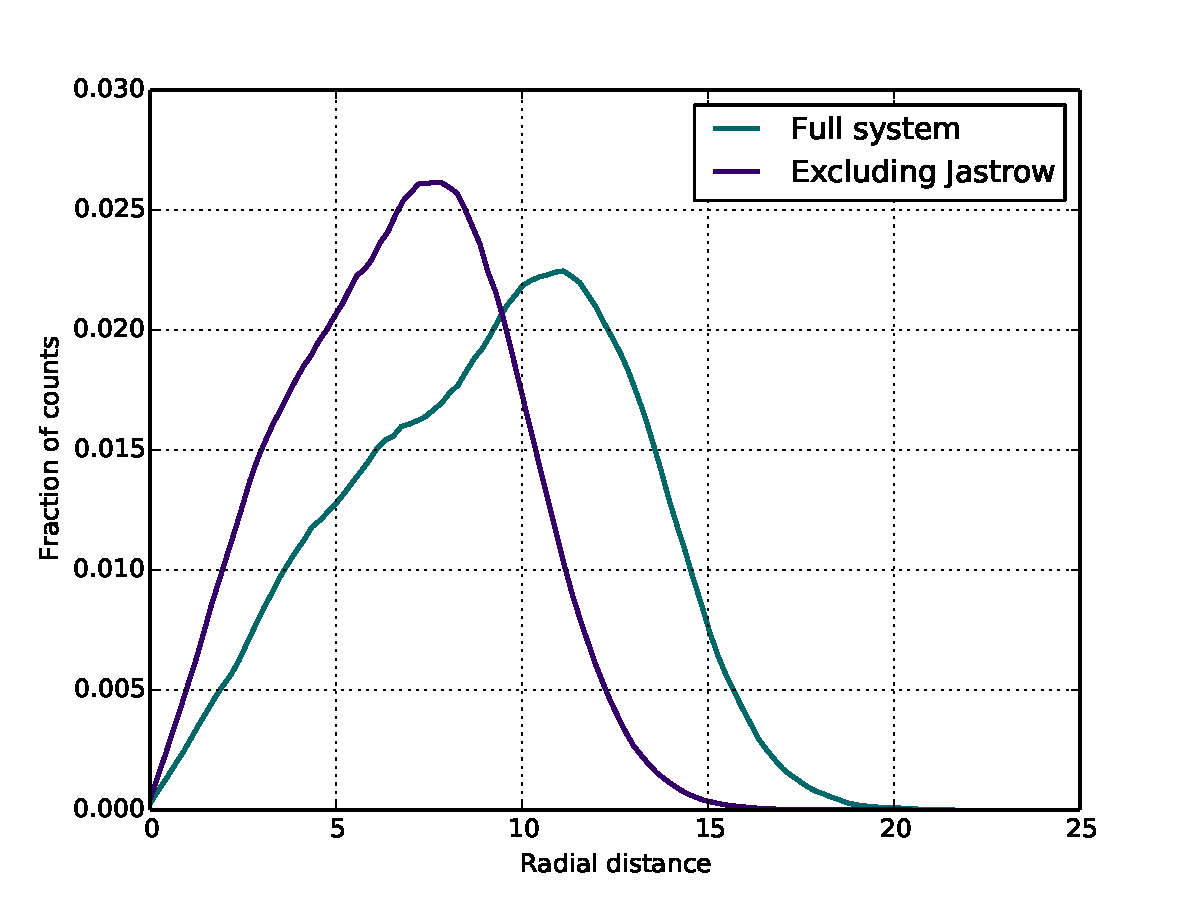
\includegraphics[width=\textwidth, height= 5cm]{figures/radialDistribution/radialDistributionN20w10Se7.pdf}
		\caption{$N=20,\:\omega=0.1$}
	\end{subfigure}
	
	\vspace{3mm}
	
	\caption{One-body densities (left) and radial distributions (right) for $N=\{2,6,12,20\}$ and $\omega = 1.0$.}
	\label{fig:Onebody&RadialDist}
\end{figure}











\newpage


% THIS IS SOME OLD CODE RIGHT HERE...

\begin{figure}[H]
	
	\begin{subfigure}{0.5\textwidth}
		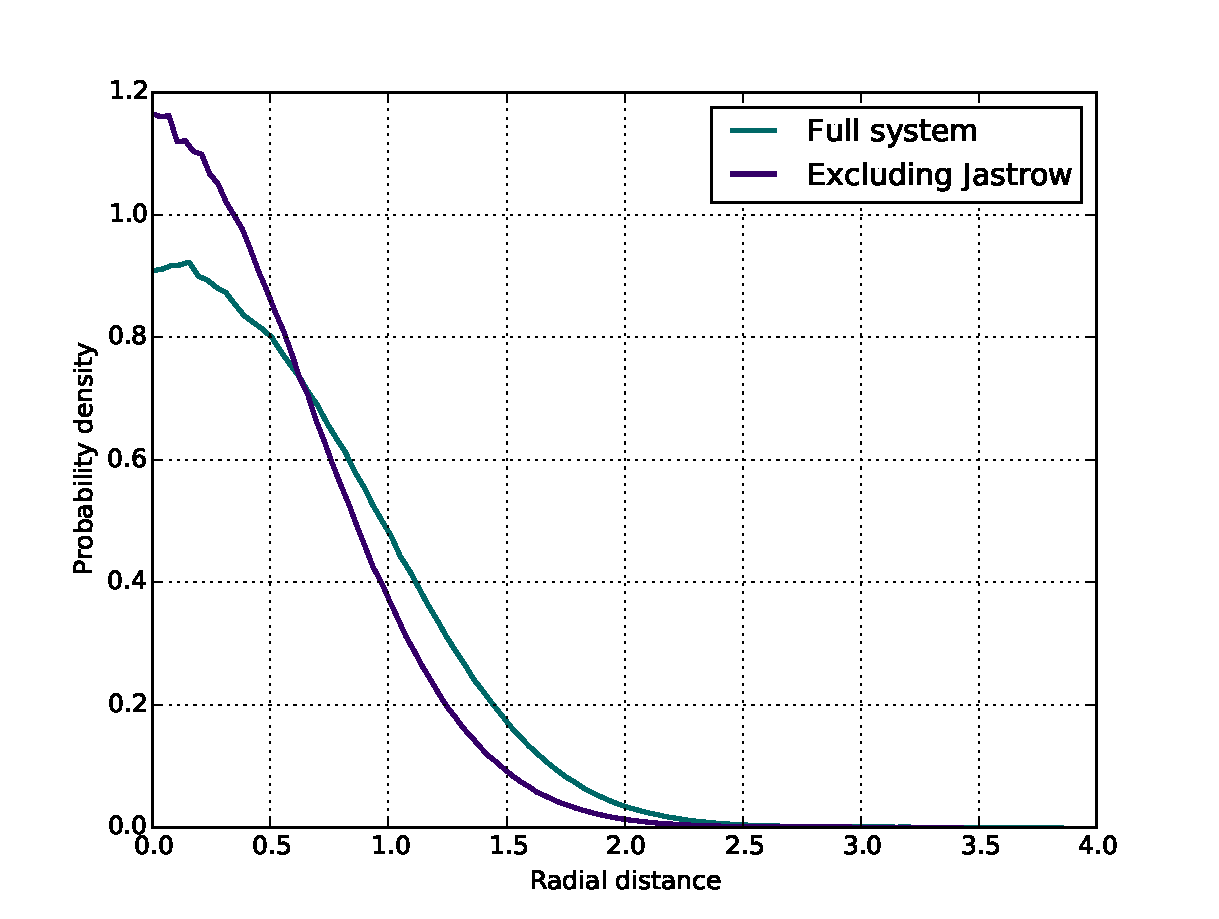
\includegraphics[width=\textwidth, height= 5cm]{figures/radialDistribution/OneBodyDensityN2w100Se7.pdf}
		\caption{$N=2,\:\omega=1.0$}
	\end{subfigure}
	\begin{subfigure}{0.5\textwidth}
		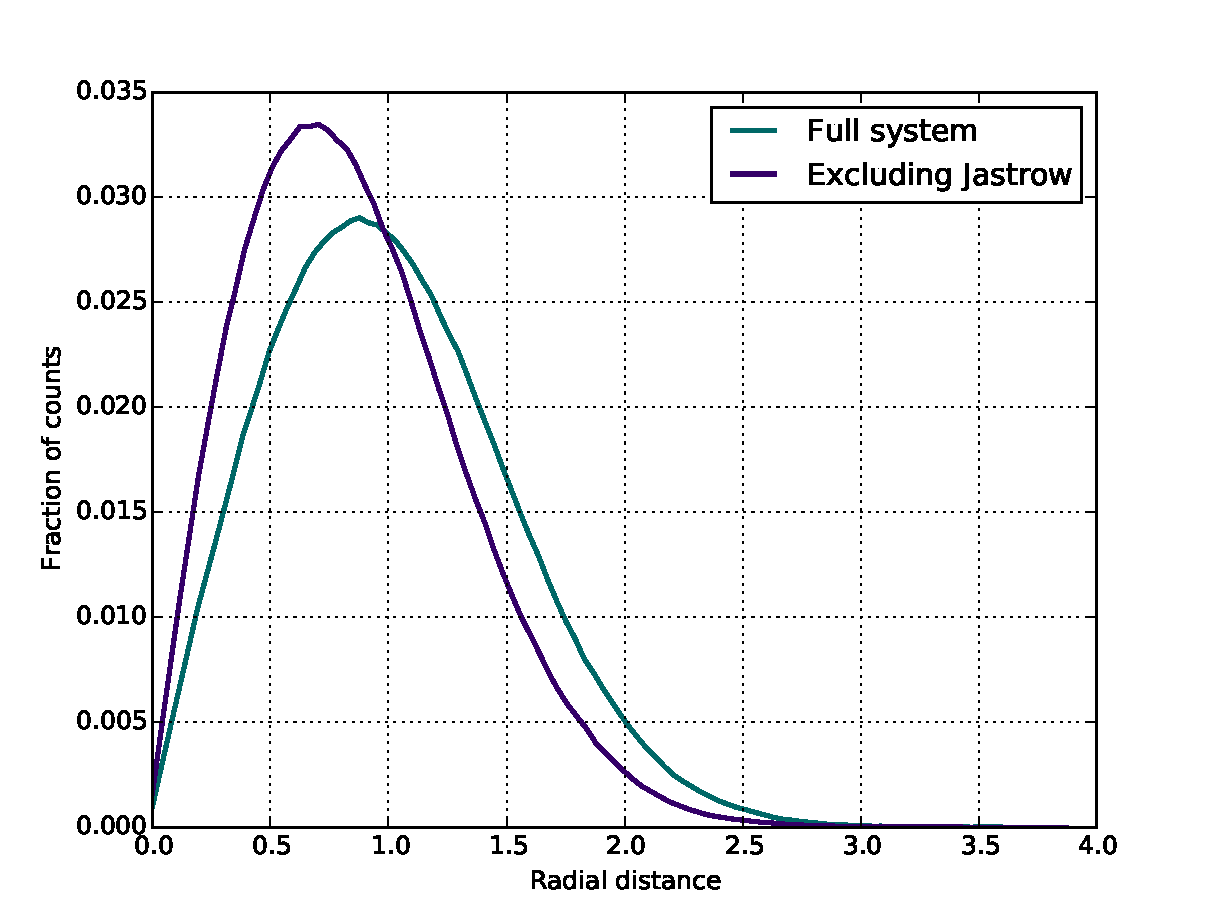
\includegraphics[width=\textwidth, height= 5cm]{figures/radialDistribution/radialDistributionN2w100Se7.pdf}
		\caption{$N=2,\:\omega=1.0$}
	\end{subfigure}
	
	\vspace{1mm}
	
	\begin{subfigure}{0.5\textwidth}
		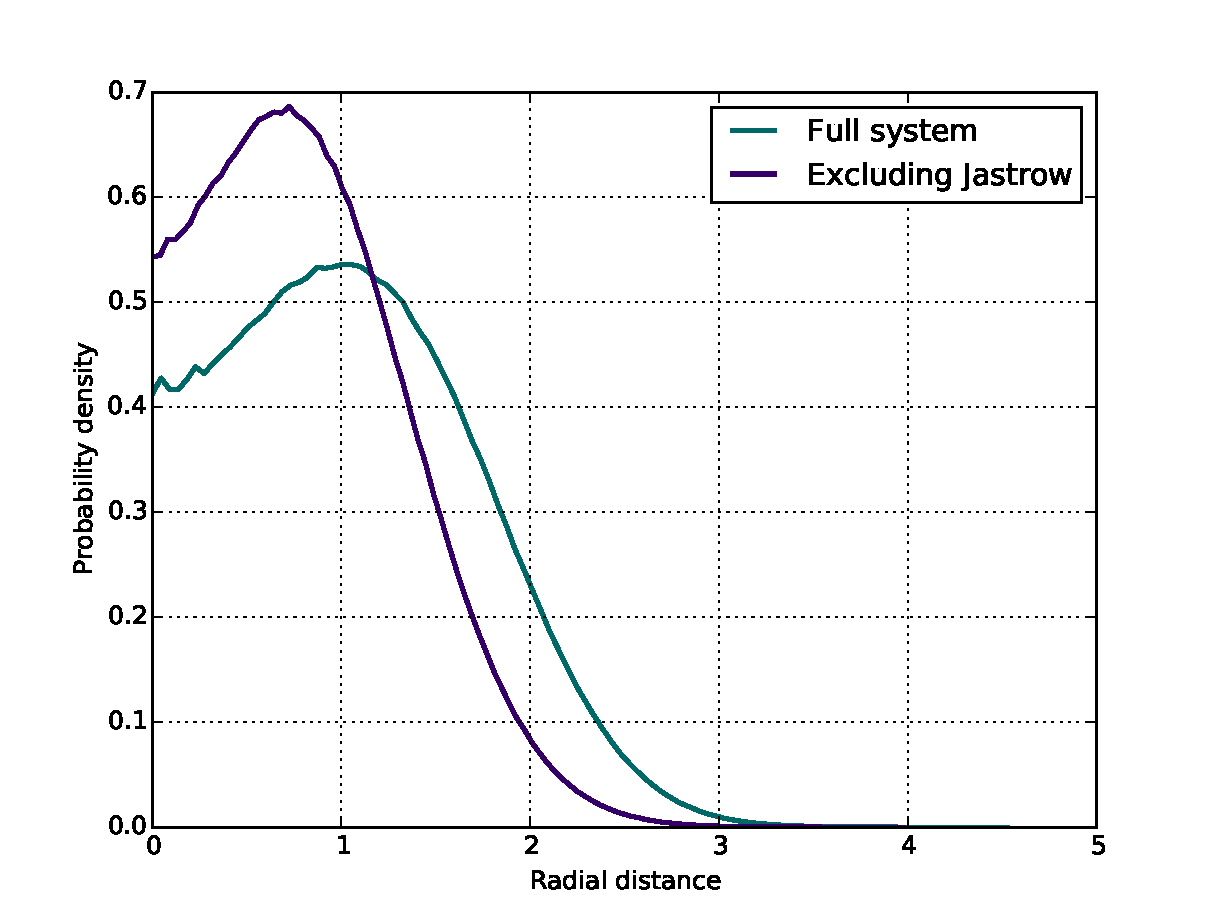
\includegraphics[width=\textwidth, height= 5cm]{figures/radialDistribution/OneBodyDensityN6w100Se7.pdf}
		\caption{$N=6,\:\omega=1.0$}
	\end{subfigure}
	\begin{subfigure}{0.5\textwidth}
		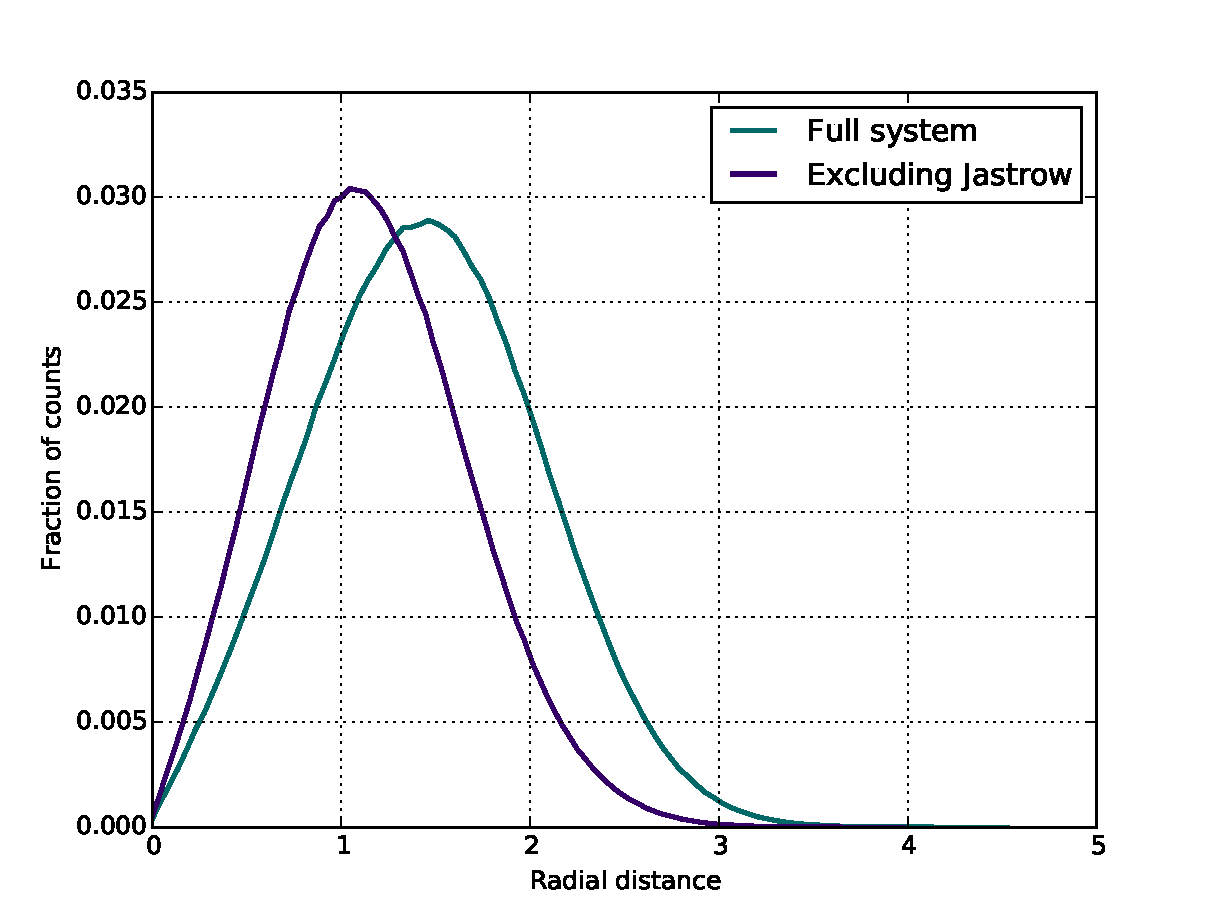
\includegraphics[width=\textwidth, height= 5cm]{figures/radialDistribution/radialDistributionN6w100Se7.pdf}
		\caption{$N=6,\:\omega=1.0$}
	\end{subfigure}
	
	\vspace{1mm}
	
	\begin{subfigure}{0.5\textwidth}
		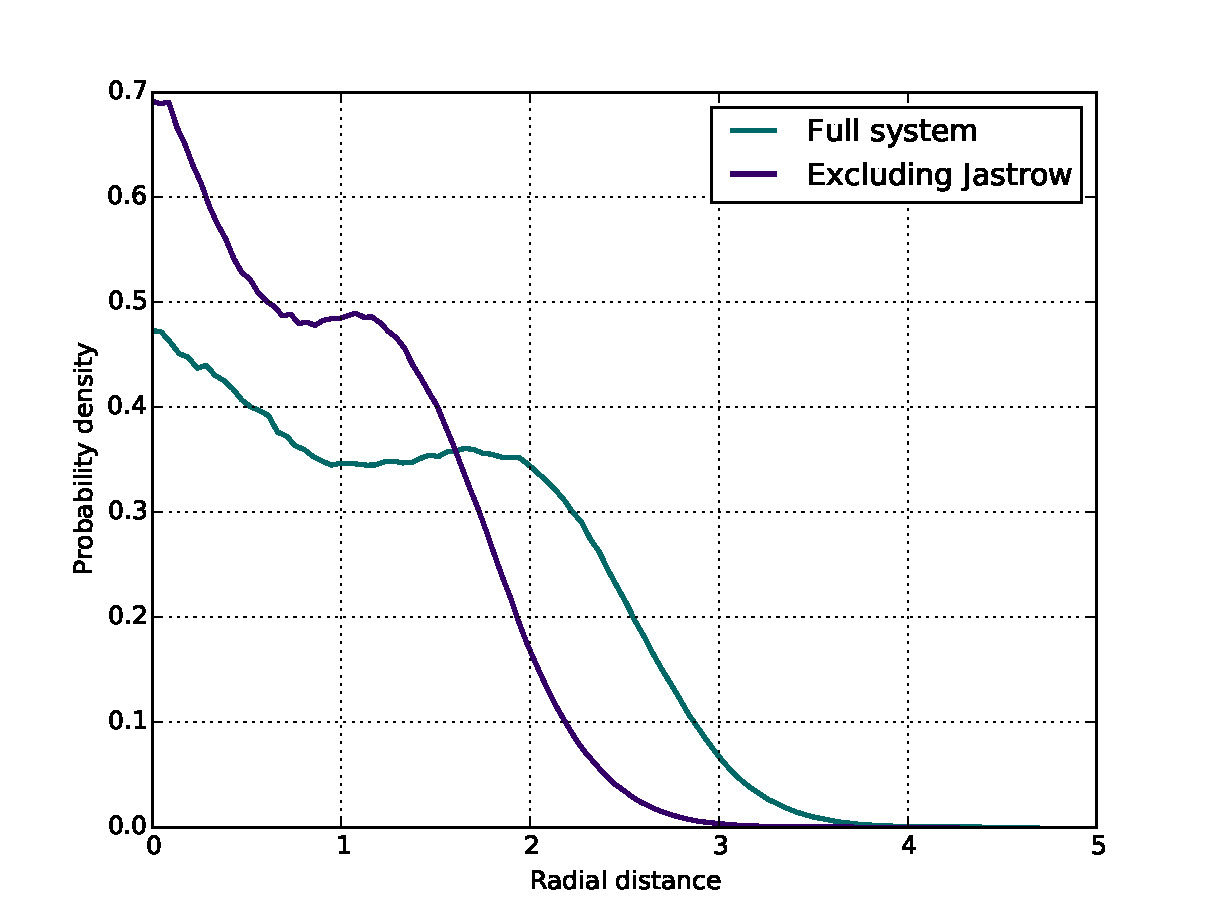
\includegraphics[width=\textwidth, height=5cm]{figures/radialDistribution/OneBodyDensityN12w100Se7.pdf}
		\caption{$N=12,\:\omega=1.0$}
	\end{subfigure}
	\begin{subfigure}{0.5\textwidth}
		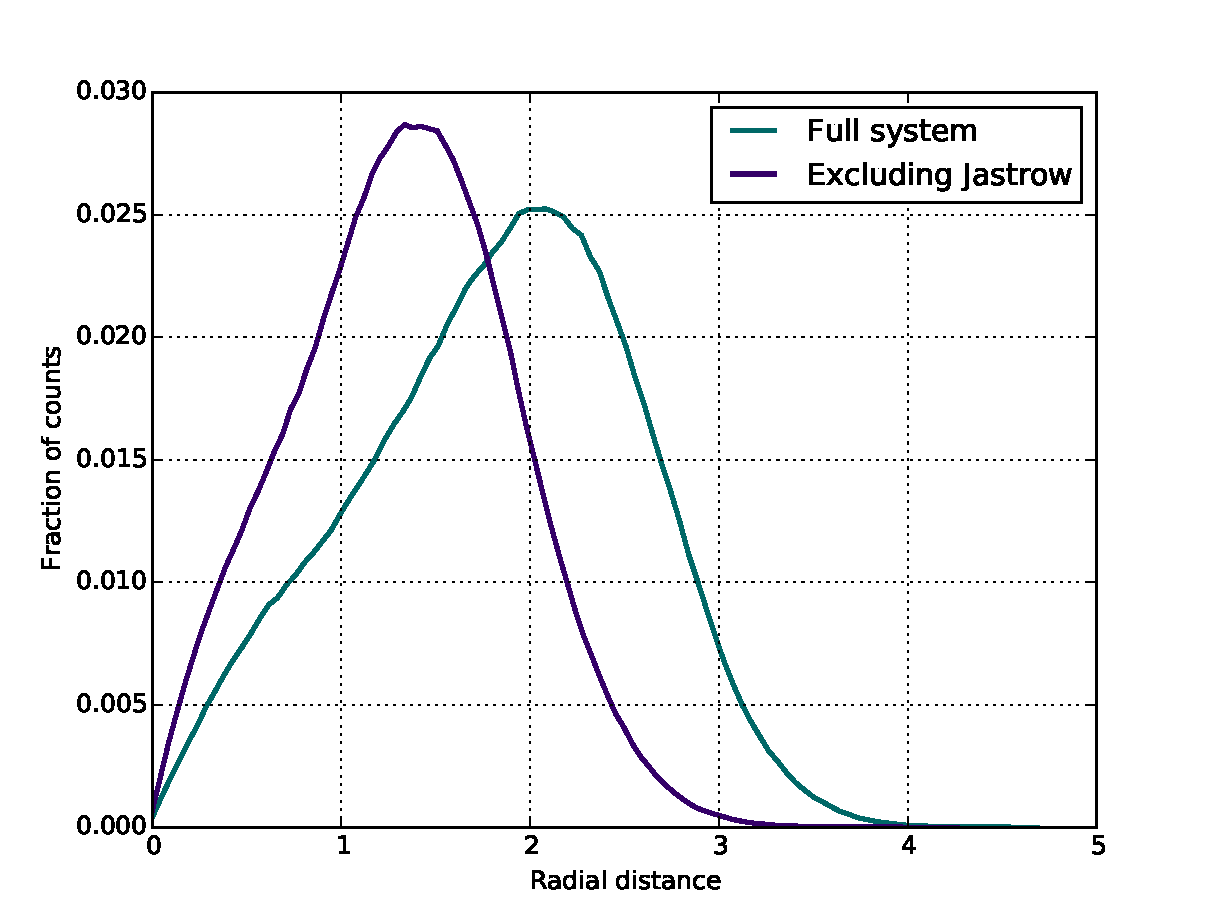
\includegraphics[width=\textwidth, height= 5cm]{figures/radialDistribution/radialDistributionN12w100Se7.pdf}
		\caption{$N=12,\:\omega=1.0$}
	\end{subfigure}
	
	\vspace{1mm}
	
	\begin{subfigure}{0.5\textwidth}
		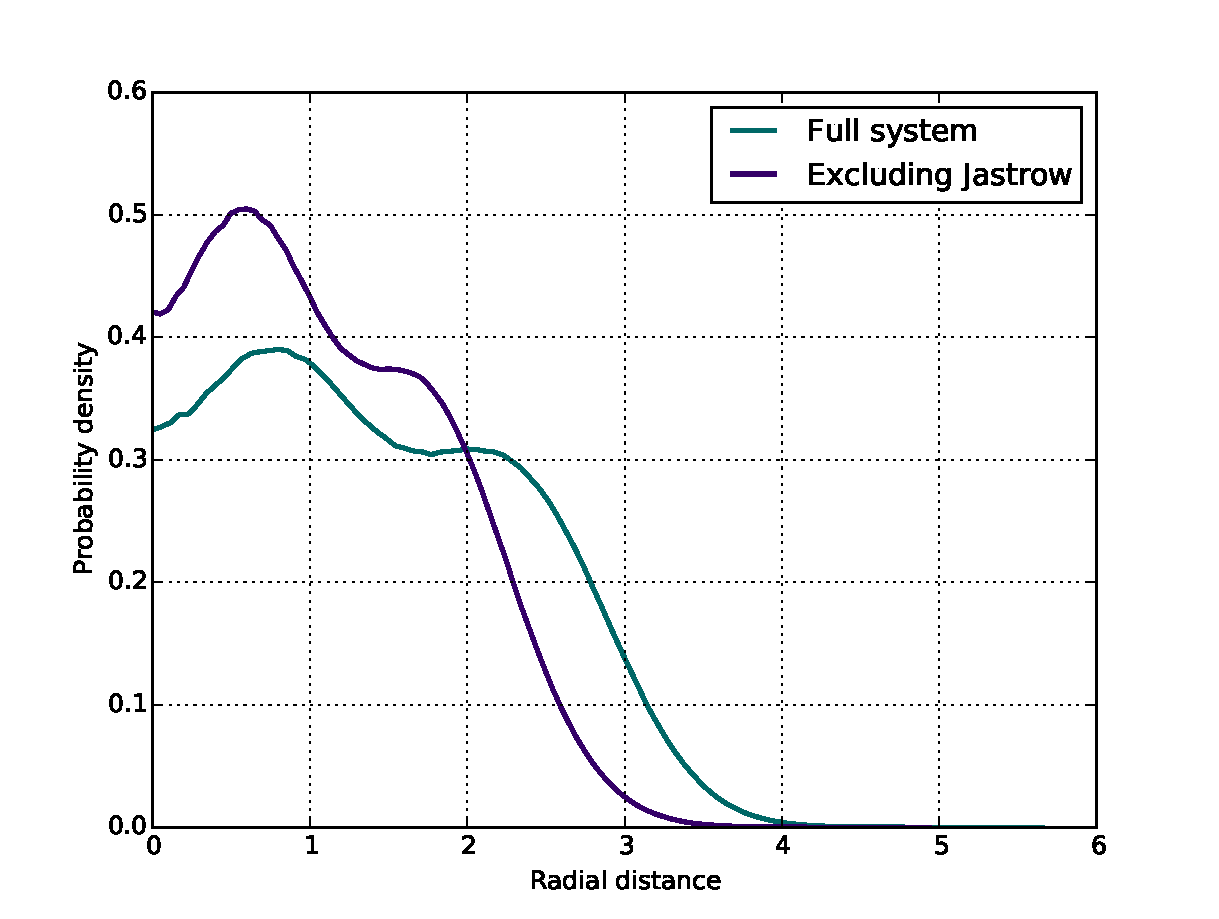
\includegraphics[width=\textwidth, height= 5cm]{figures/radialDistribution/OneBodyDensityN20w100Se8.pdf}
		\caption{$N=20,\:\omega=1.0$}
	\end{subfigure}
	\begin{subfigure}{0.5\textwidth}
		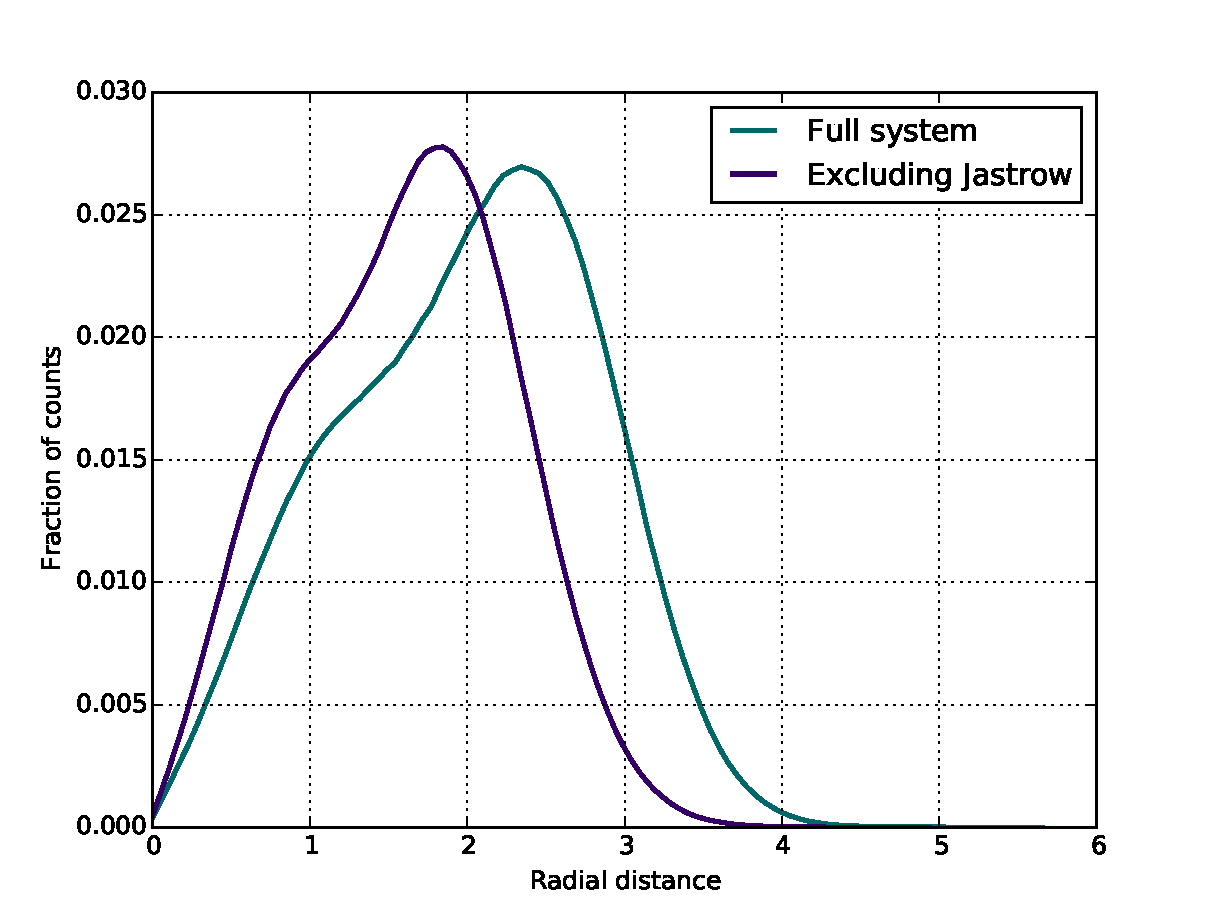
\includegraphics[width=\textwidth, height= 5cm]{figures/radialDistribution/radialDistributionN20w100Se8.pdf}
		\caption{$N=20,\:\omega=1.0$}
	\end{subfigure}
	
	\vspace{3mm}
	
	\caption{One-body densities (left) and radial distributions (right) for $N=\{2,6,12,20\}$ and $\omega = 1.0$.}
	\label{fig:Onebody&RadialDist}
\end{figure}









	
	\section{Comments}
	How to start?
	
\end{document}